\section{Evaluation}
\label{sec:evaluation}

This section evaluates ALC as a compiler transformation by applying data permutation to a set of control-divergent loops and comparing its effectiveness to previous implementations of ALC and to code generated by existing production compilers. 
This evaluation aims to answer the following questions:

\noindent\circled{1} Can Data Permutation improve ALC performance by reducing memory stalls?

\noindent\circled{2} Do scatter instructions impact ALC's performance?

\noindent\circled{3} Should ALC be applied on loops with a single \cpath?

The results indicate that data permutation leads to a significant speedup of up to 79\% over \ifconverted code and outperforms state-of-the-art compiler-based approaches.

\subsection{Setup}
\label{sec:setup}

The experiments run on a machine equipped with a Fujitsu A64FX locked at $1.8$GHz that has access to 32GiB of RAM and runs Rocky Linux (release 8.4).
A64FX is the first processor that implements ARMv8.2-A SVE instruction and it operates with 512-bit vector registers.
The evaluation micro-benchmarks were developed in-house and are written in the C language.
Each micro-benchmark is designed to be representative of application code and to ease the identification and measurement of factors that impact the performance of both \ifconverted code and ALC-transformed code.
Wyatt \etal seminal work predicted the performance of ALC using hand-modified versions of applications in the SPEC CPU2017 benchmark suite running on a functional simulator~\cite{spec}.
Those modifications included removing control-flow dependent paths that execute I/O operations --- a transformation that cannot be safely implemented in a compiler because it alters the behavior of the program.
This work aims to evaluate the automated generation of ALC code by a compiler transformation pass and thus can only be applied to programs to which the compiler can safely apply ALC without user intervention.
The micro-benchmarks used in this evaluation are comprehensive and share characteristics with loops found in the SPEC CPU2017 benchmark Suite.
The limitations and challenges of the current ALC implementation are discussed in \rsec{eval-limitations}.

The evaluation micro-benchmarks consist of loops that contain either an \code{if-then-else} or  a single \code{if} statement.
Two micro-benchmarks help understand the impact of the factors discussed in \rsec{alc-analysis}:
\begin{inparaenum}
    \item \textbf{\ifElseBench} contains a loop that executes $N$ times with two \cpaths in its body. Each \cpath has: $20$ arithmetic, $2$ load, and $3$ store instructions;
    \item \textbf{\ifThenBench} also contains a loop that executes $N$ times but with a single \cpath, which has: $20$ arithmetic, $2$ load, and $3$ store instructions.
\end{inparaenum}
$N$ is set to five million for all experiments.
Complete source code of ALC's LLVM IR pass and evaluation micro-benchmarks is available as part of this paper's \textbf{ARTIFACT}\footnote{\textbf{link omitted due to double-blind reviews.}}.
All source code is compiled with Clang/LLVM version 15.0.0\footnote{\href{https://github.com/llvm/llvm-project/commit/61baf2ffa7071944c00a0642fdb9ff77d9cff0da}{61baf2ffa7071944c00a0642fdb9ff77d9cff0da}} and highest optimization level enabled (\code{-O3}).


\begin{figure*}[t]
  \centering
  \begin{subfigure}{4cm}
    \centering
    
\includegraphics[width=\textwidth]{Figures/Evaluations/Legend.png}
  \end{subfigure}\\
  \begin{subfigure}{.36\textwidth}
    \centering
    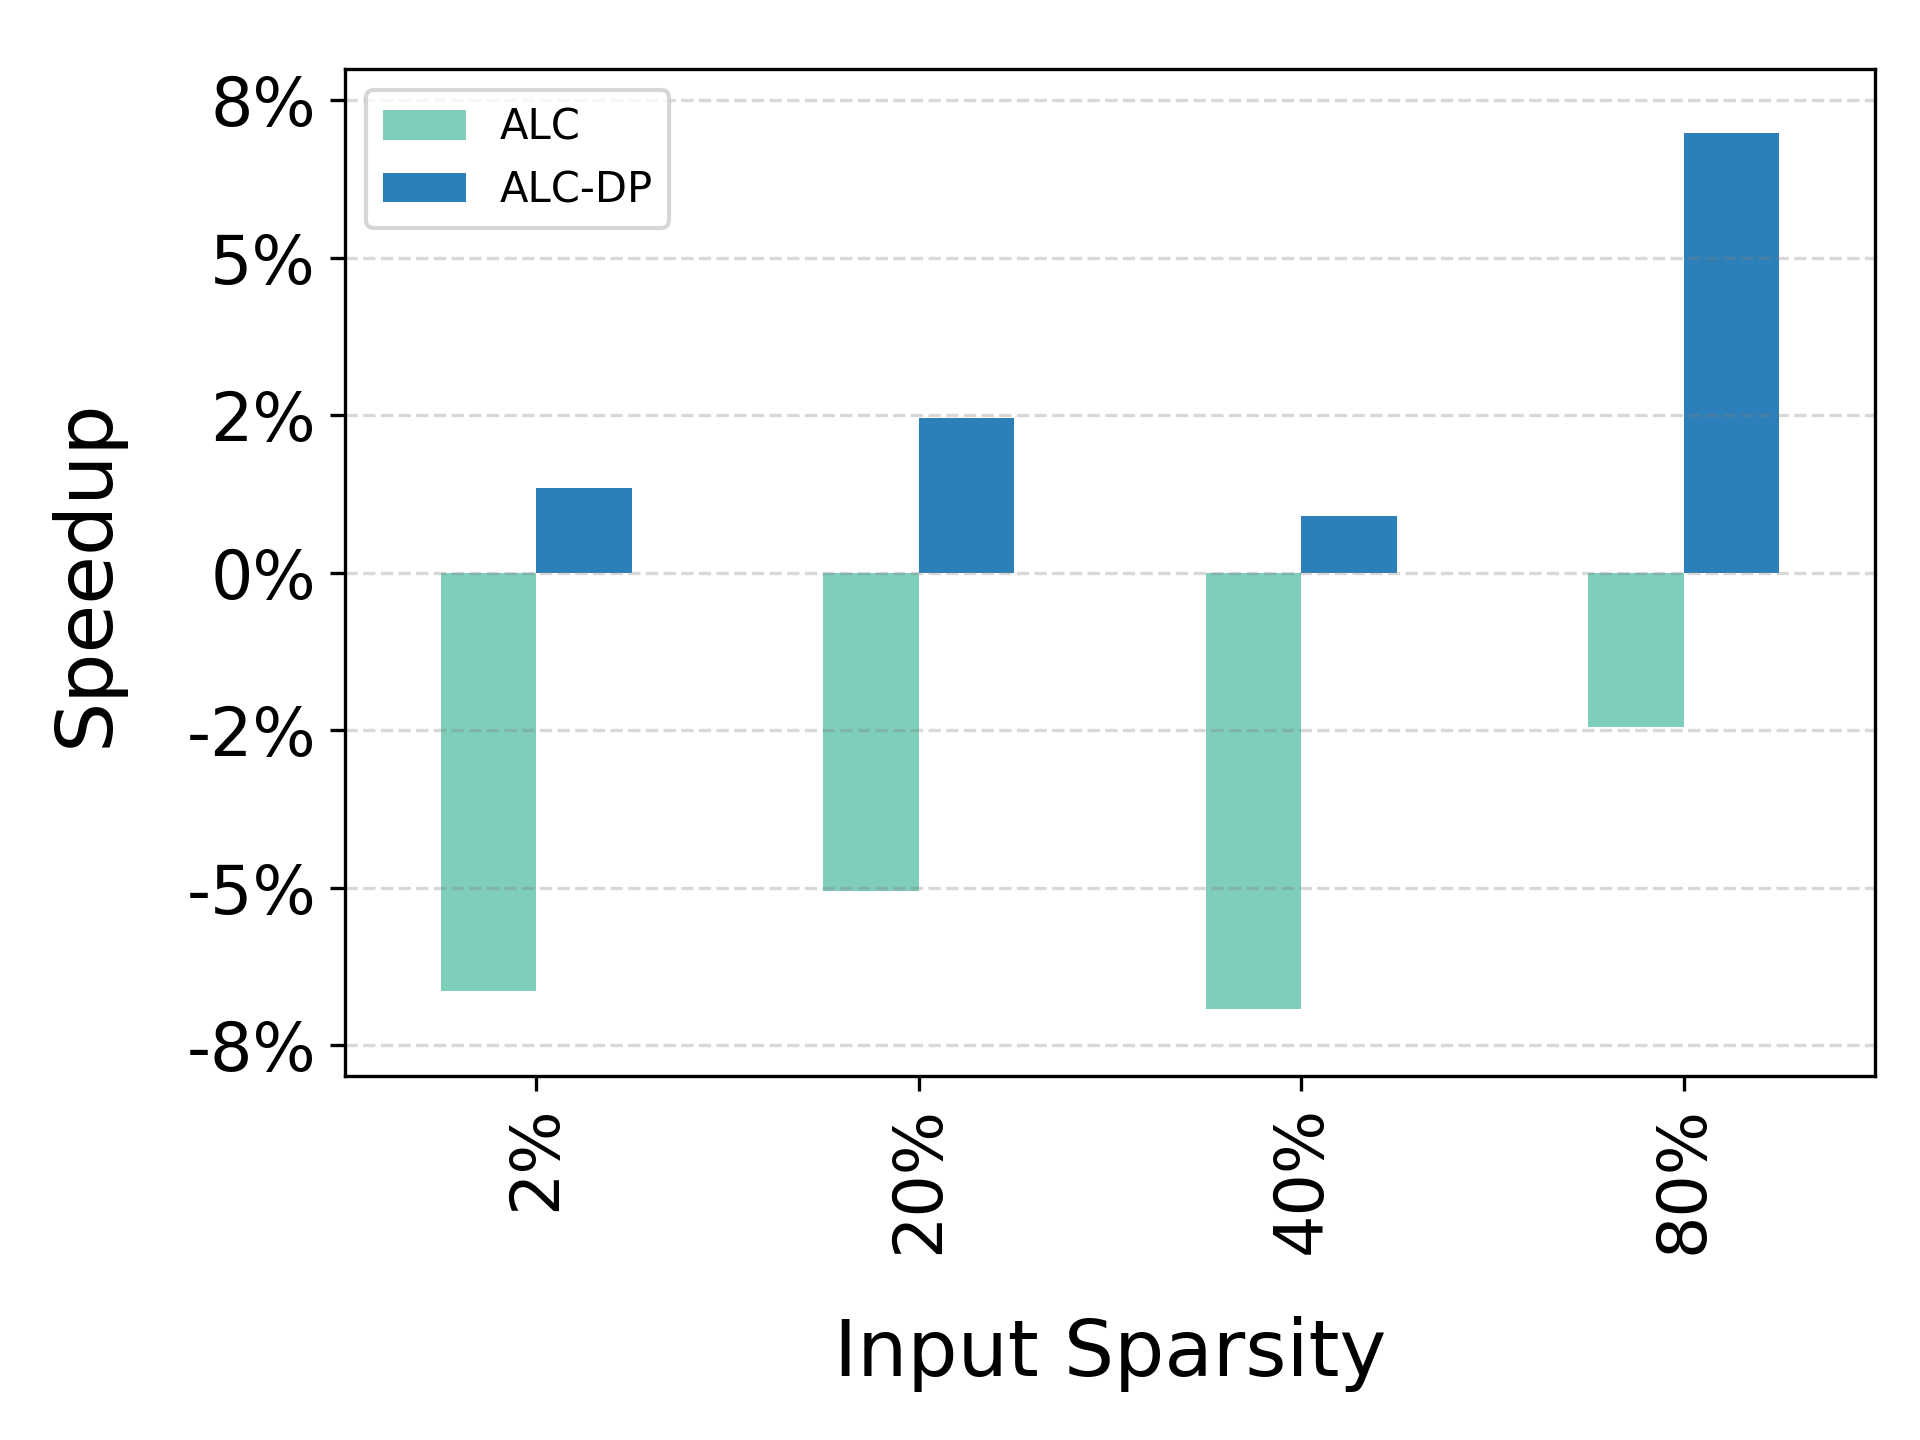
\includegraphics[width=\textwidth]{Figures/Evaluations/if_then_else_many_scatter_speedup.png}
    \caption{Speedup over \ifconverted code (\ifconv).}
     \label{fig:if-then-else-many-scatter-speedup}
  \end{subfigure}%
  \begin{subfigure}{.36\textwidth}
        \centering
    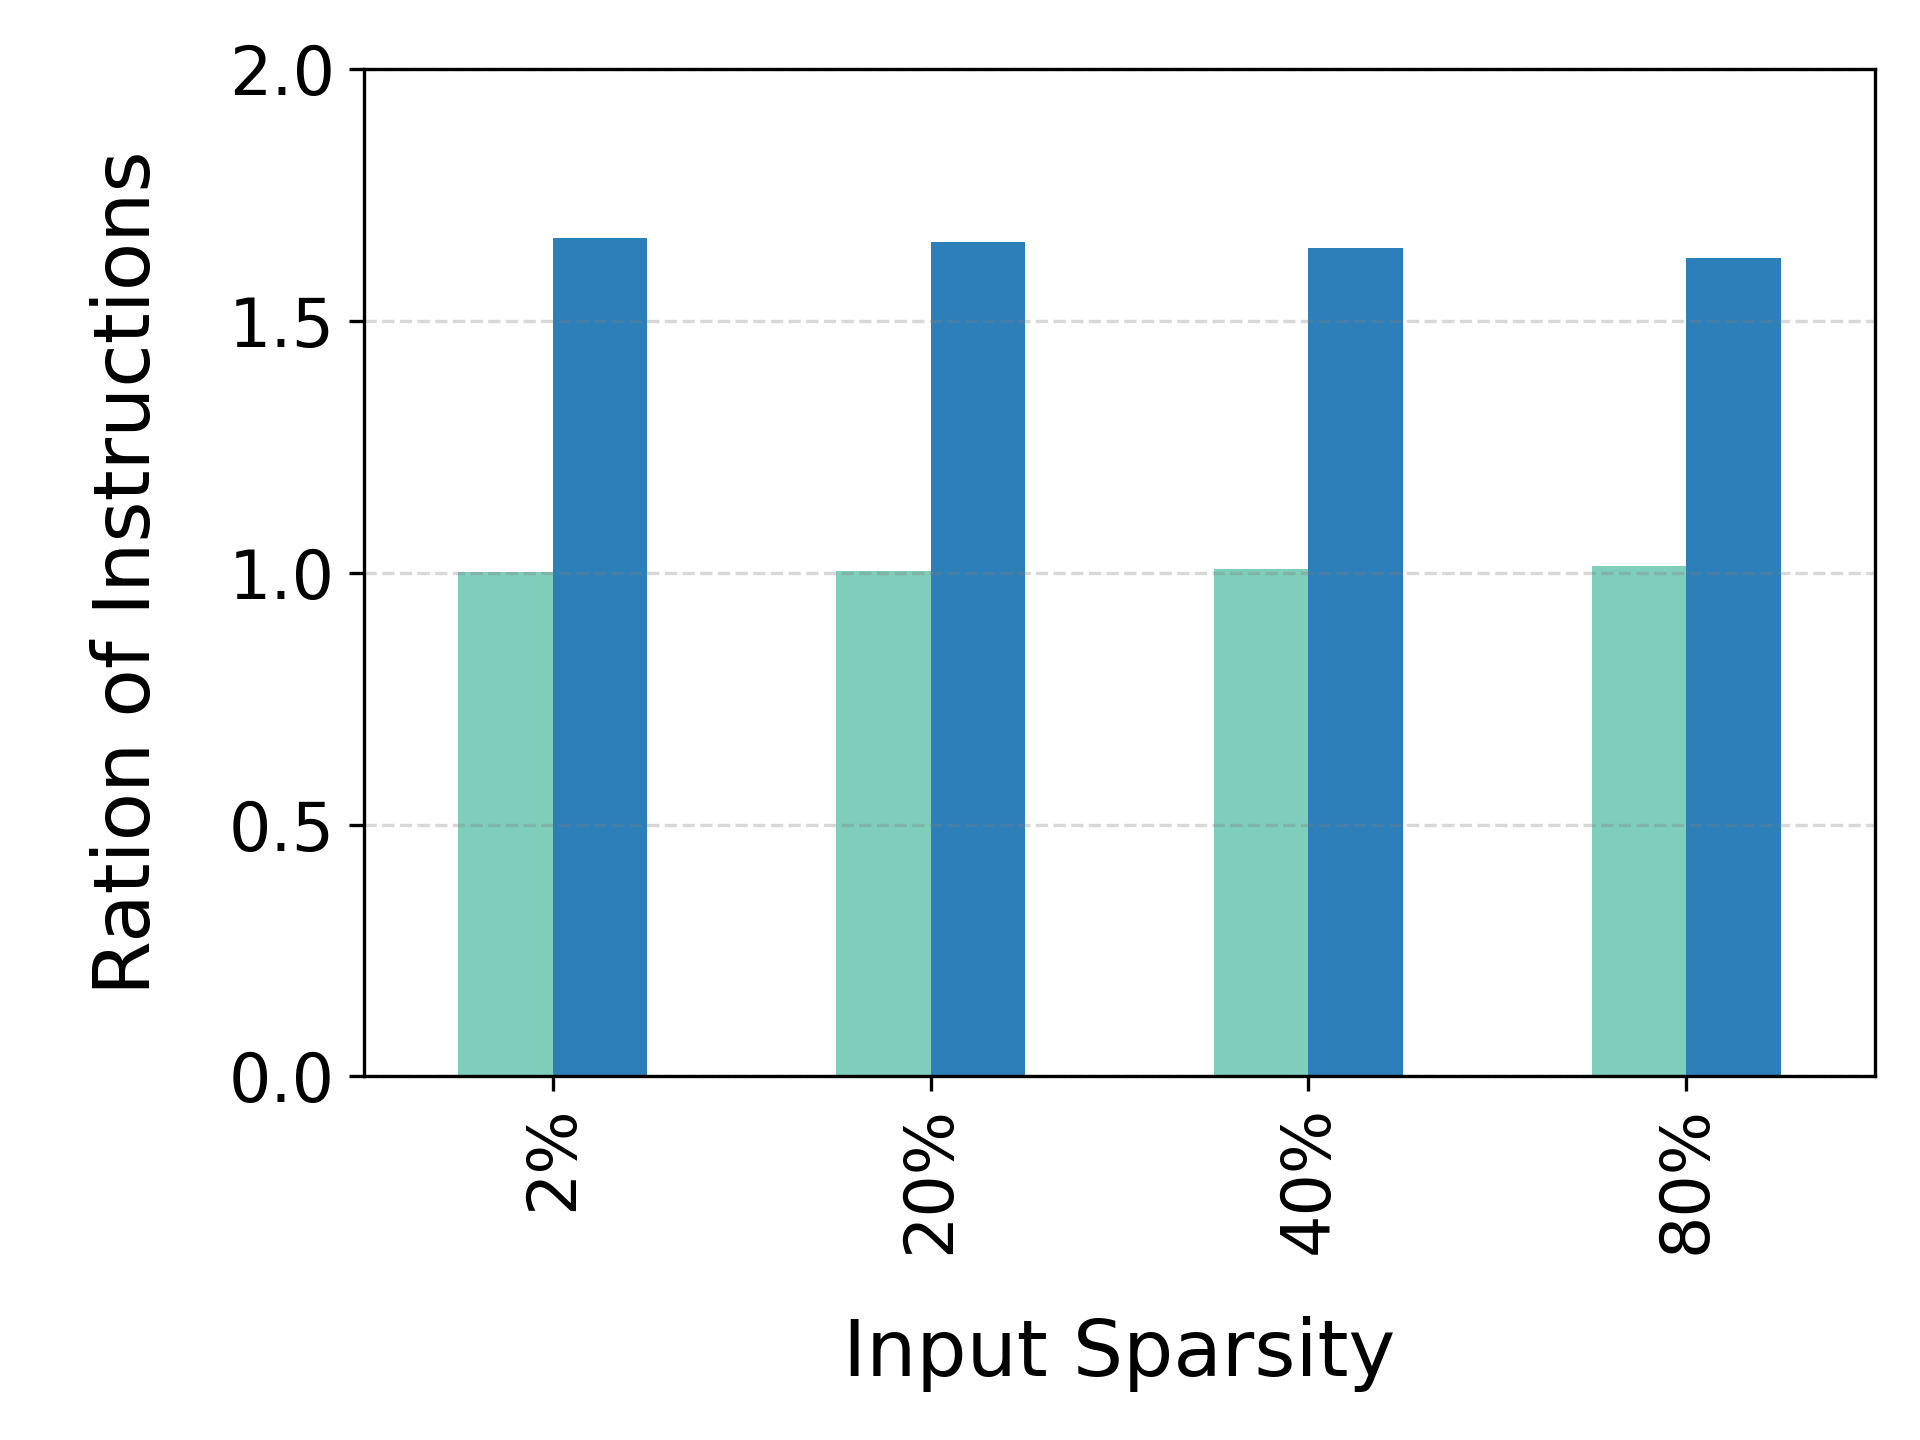
\includegraphics[width=\textwidth]{Figures/Evaluations/if_then_else_many_scatter_instr.png}
    \caption{Normalized number of executed instructions.}
    \label{fig:if-then-else-many-scatter-inst}
  \end{subfigure}
  \begin{subfigure}{.36\textwidth}
    \centering
    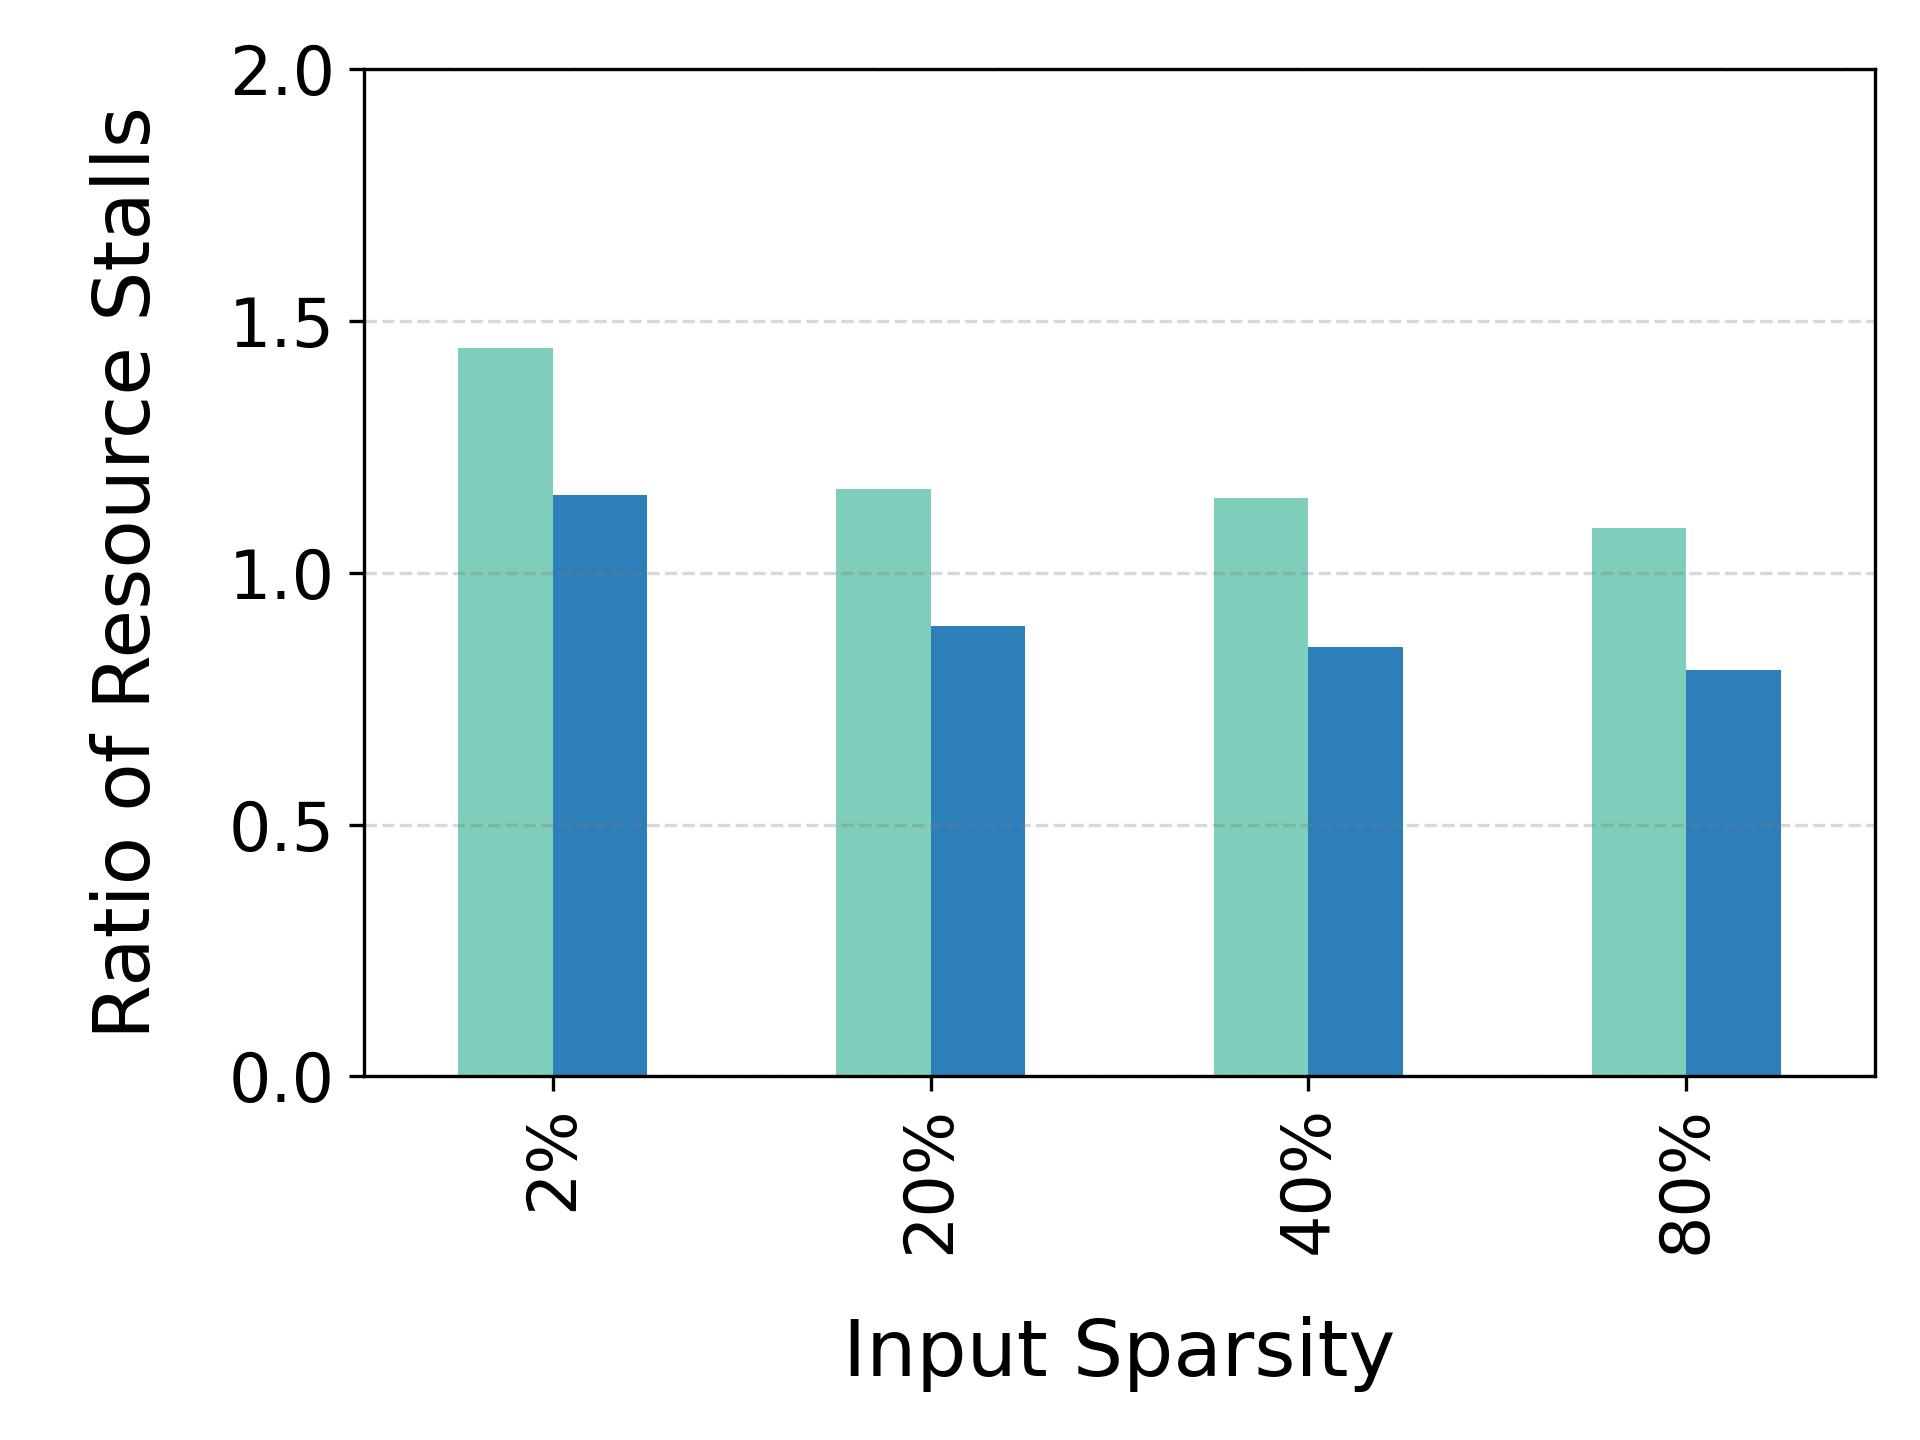
\includegraphics[width=\textwidth]{Figures/Evaluations/if_then_else_many_scatter_resource_stalls.png}
    \caption{Ratio of resource-busy stalls.}
    \label{fig:if-then-else-many-scatter-resource}
  \end{subfigure}%
  \begin{subfigure}{.36\textwidth}
        \centering
    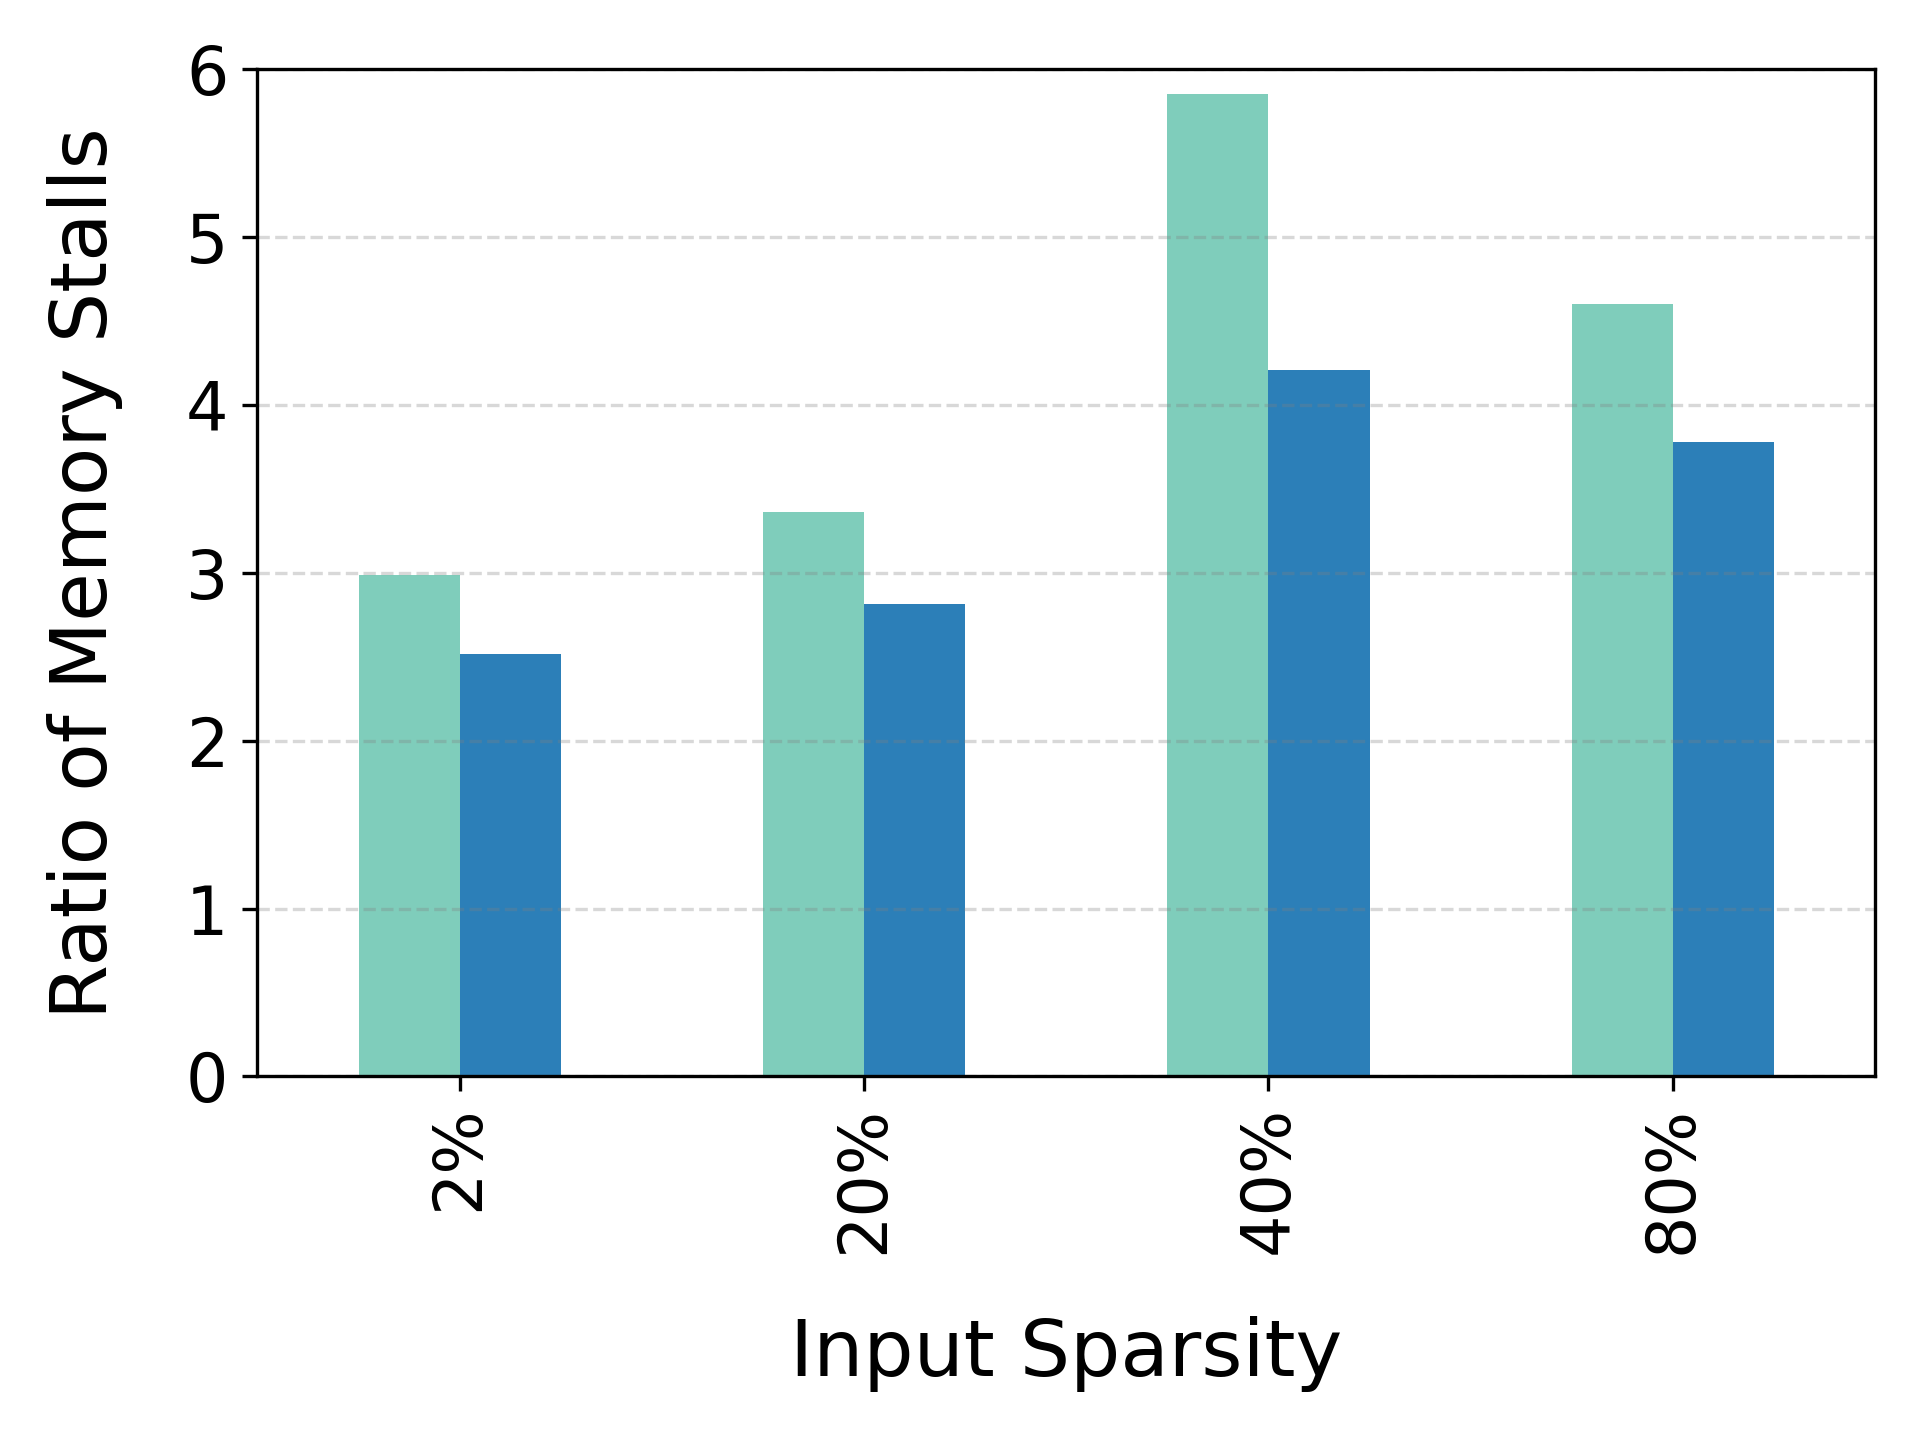
\includegraphics[width=\textwidth]{Figures/Evaluations/if_then_else_many_scatter_mem_stalls.png}
    \caption{Ratio of memory-induced stalls.}
    \label{fig:if-then-else-many-scatter-mem-stalls}
  \end{subfigure}%
  \caption{Evaluation of the \ifElseBench micro-benchmark that has two CFDPs. All metrics are normalized with respect to \ifconverted code (\ifconv).}
\end{figure*}

\subsection{Experimental Methodology}
\label{sec:methodology}

Results presented in the following sections are the average of one hundred executions of each program.
Very little variation was observed between measurements.
Performance metrics were collected using PAPI library version $7.0.0$\footnote{\href{https://bitbucket.org/icl/papi/commits/c415d2f1190027c961c904a4305b3eeaacce3df2}{c415d2f1190027c961c904a4305b3eeaacce3df2}}~\cite{papi}.
The performance for each micro-benchmark is measured with varied \textbf{input sparsity}, the percentage of loop iterations in which the control-flow condition evaluates to true.
Results are reported for input sparsity of $2\%$, $20\%$, $40\%$, and $80\%$, with true predicates randomly distributed throughout the loop iterations.
These percentages represent use cases varying from very few active lanes ($2\%$) to mostly active lanes ($80\%$).
A random distribution of true predicates means that none of the evaluated approaches can make assumptions about the order or the pattern of taken/not-taken paths.
To Apply ALC, input source code is first compiled to LLVM IR using Clang. The  produced IR is fed to the transformation pass and all analyses and transformations are done at this level. Then clean up and further optimization passes in the \code{O3} pipeline are executed to ensure that the transformed IR is fully optimized. 
Finally, the generated binary file is produced.

The results presented next contrast the performance of:
\begin{inparaenum}[(i)]
  \item \textbf{\ALC}, a compiler-generated version of Wyatt \etal's ALC;
  \item \textbf{\ALCdp}, the improved version of \ALC proposed in this work which employs data permutation to eliminate gather instructions;
  \item \textbf{\ifconv}, \ifconversion performed by Arm's Clang compiler.
\end{inparaenum}
A comparison of the \ifconversion code generated by three production-ready compilers --- Arm's Clang, GCC, and Clang --- revealed that Arm's Clang generates slightly faster code for the evaluated micro-benchmarks.


\begin{figure*}[t]
  \centering
%  \begin{subfigure}{4cm}
    %\centering
    %
\includegraphics[width=\textwidth]{Figures/Evaluations/Legend.png}
%  \end{subfigure}\\
  \begin{subfigure}{.33\textwidth}
    \centering
    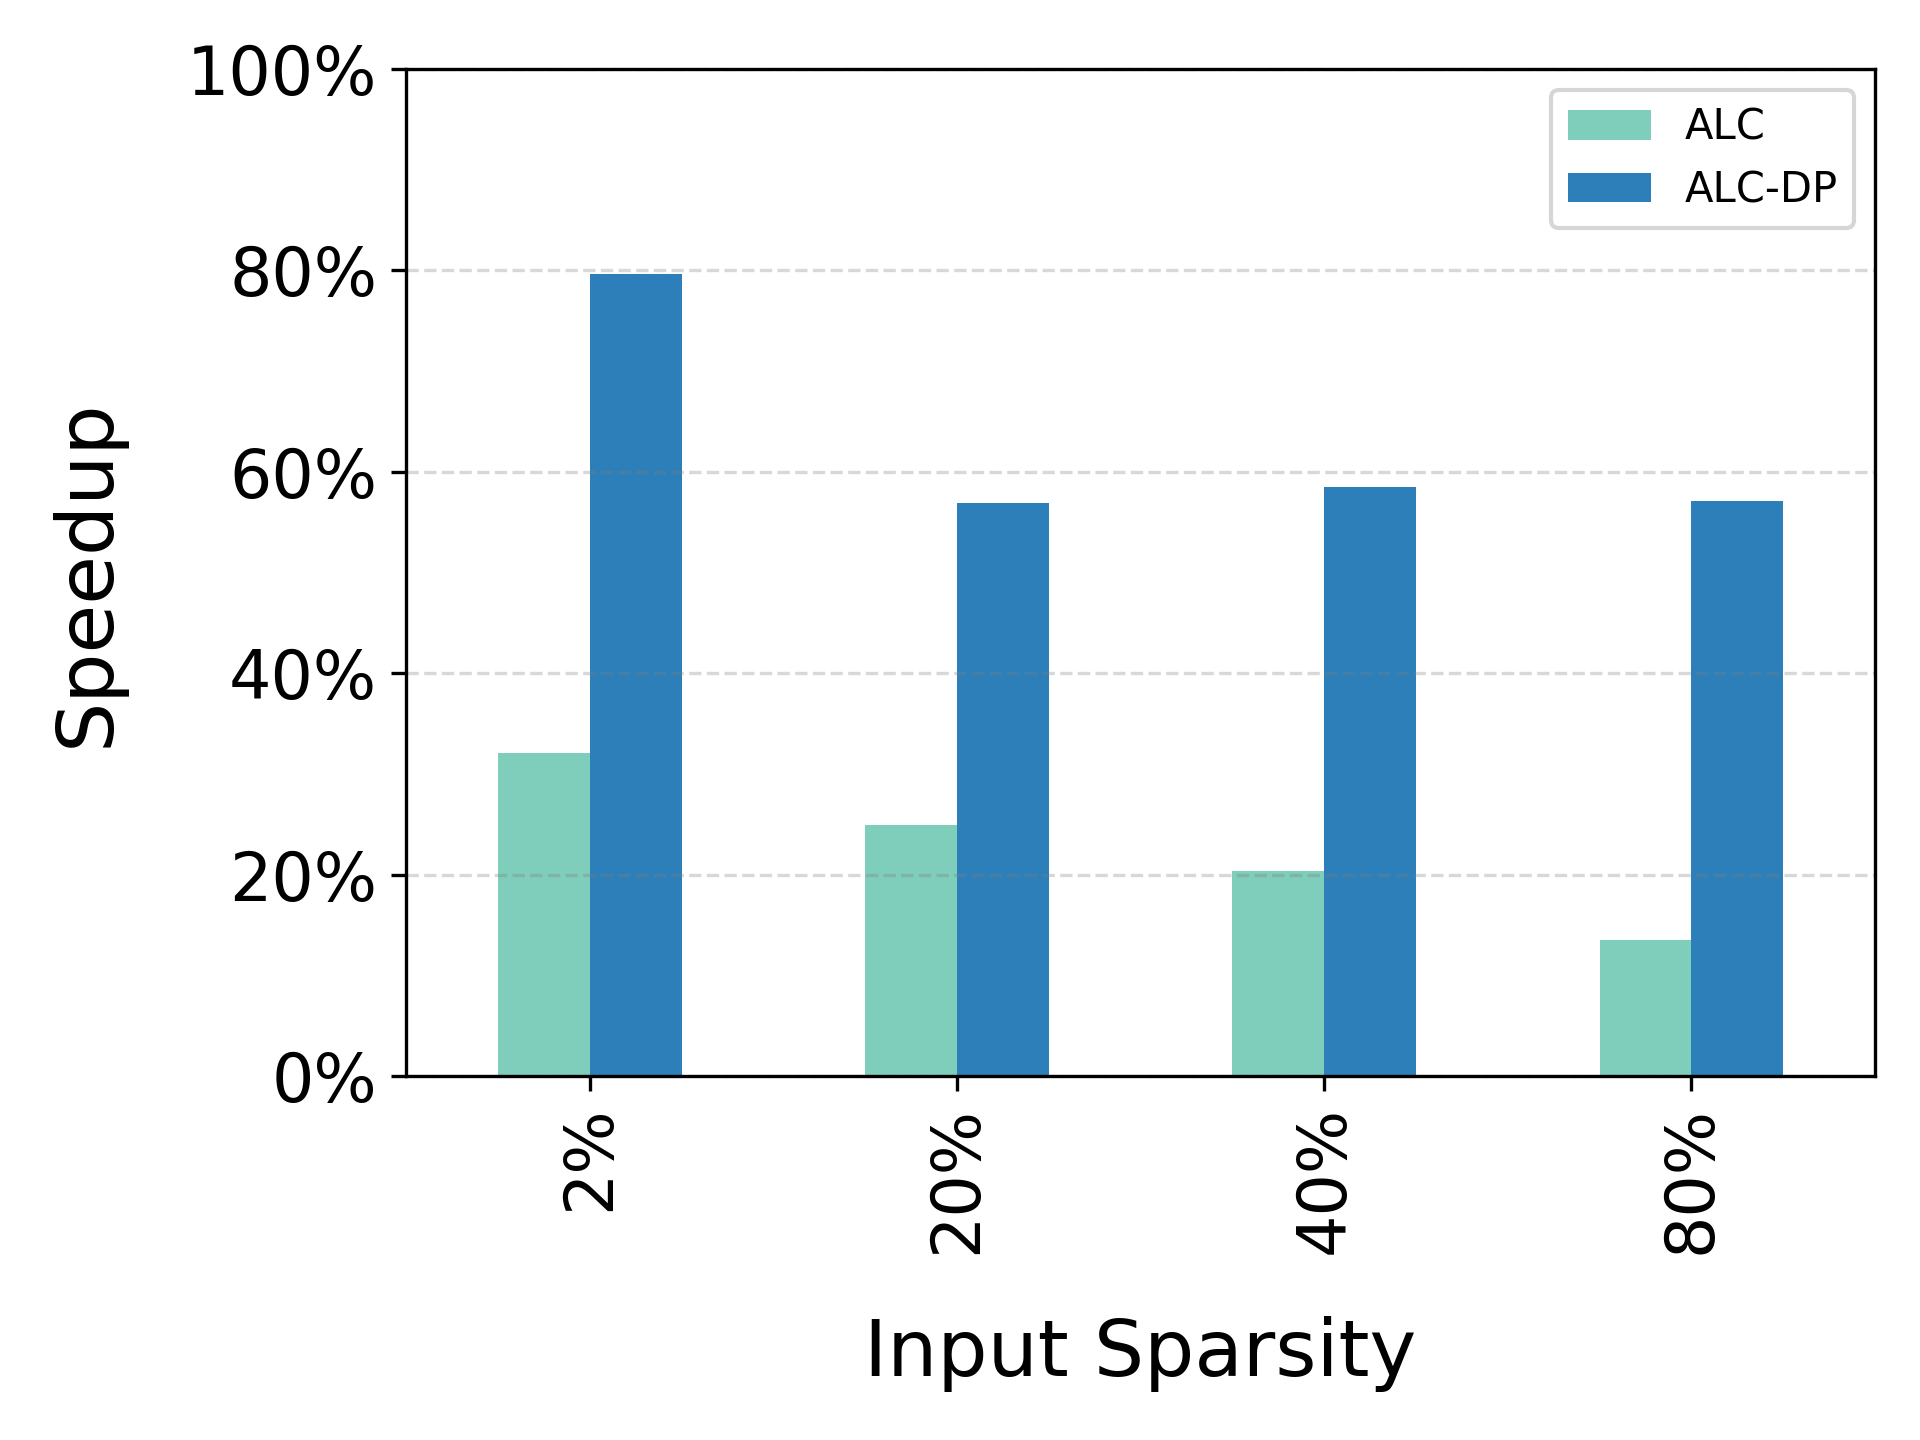
\includegraphics[width=\textwidth]{Figures/Evaluations/if_then_else_few_scatter_speedup.png}
    \caption{Speedup over \ifconv.}
     \label{fig:if-then-else-few-scatter-speedup}
  \end{subfigure}%
%  \begin{subfigure}{.4\textwidth}
%    \centering
%    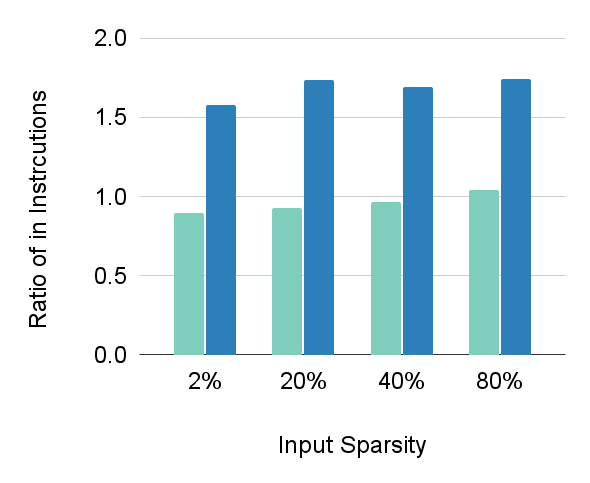
\includegraphics[width=\textwidth]{Figures/Evaluations/if_then_else_few_scatter_instr.png.png}
%    \caption{Ratio number of executed instructions.}
%    \label{fig:if-then-else-few-scatter-inst}
%  \end{subfigure}
  \begin{subfigure}{.33\textwidth}
    \centering
    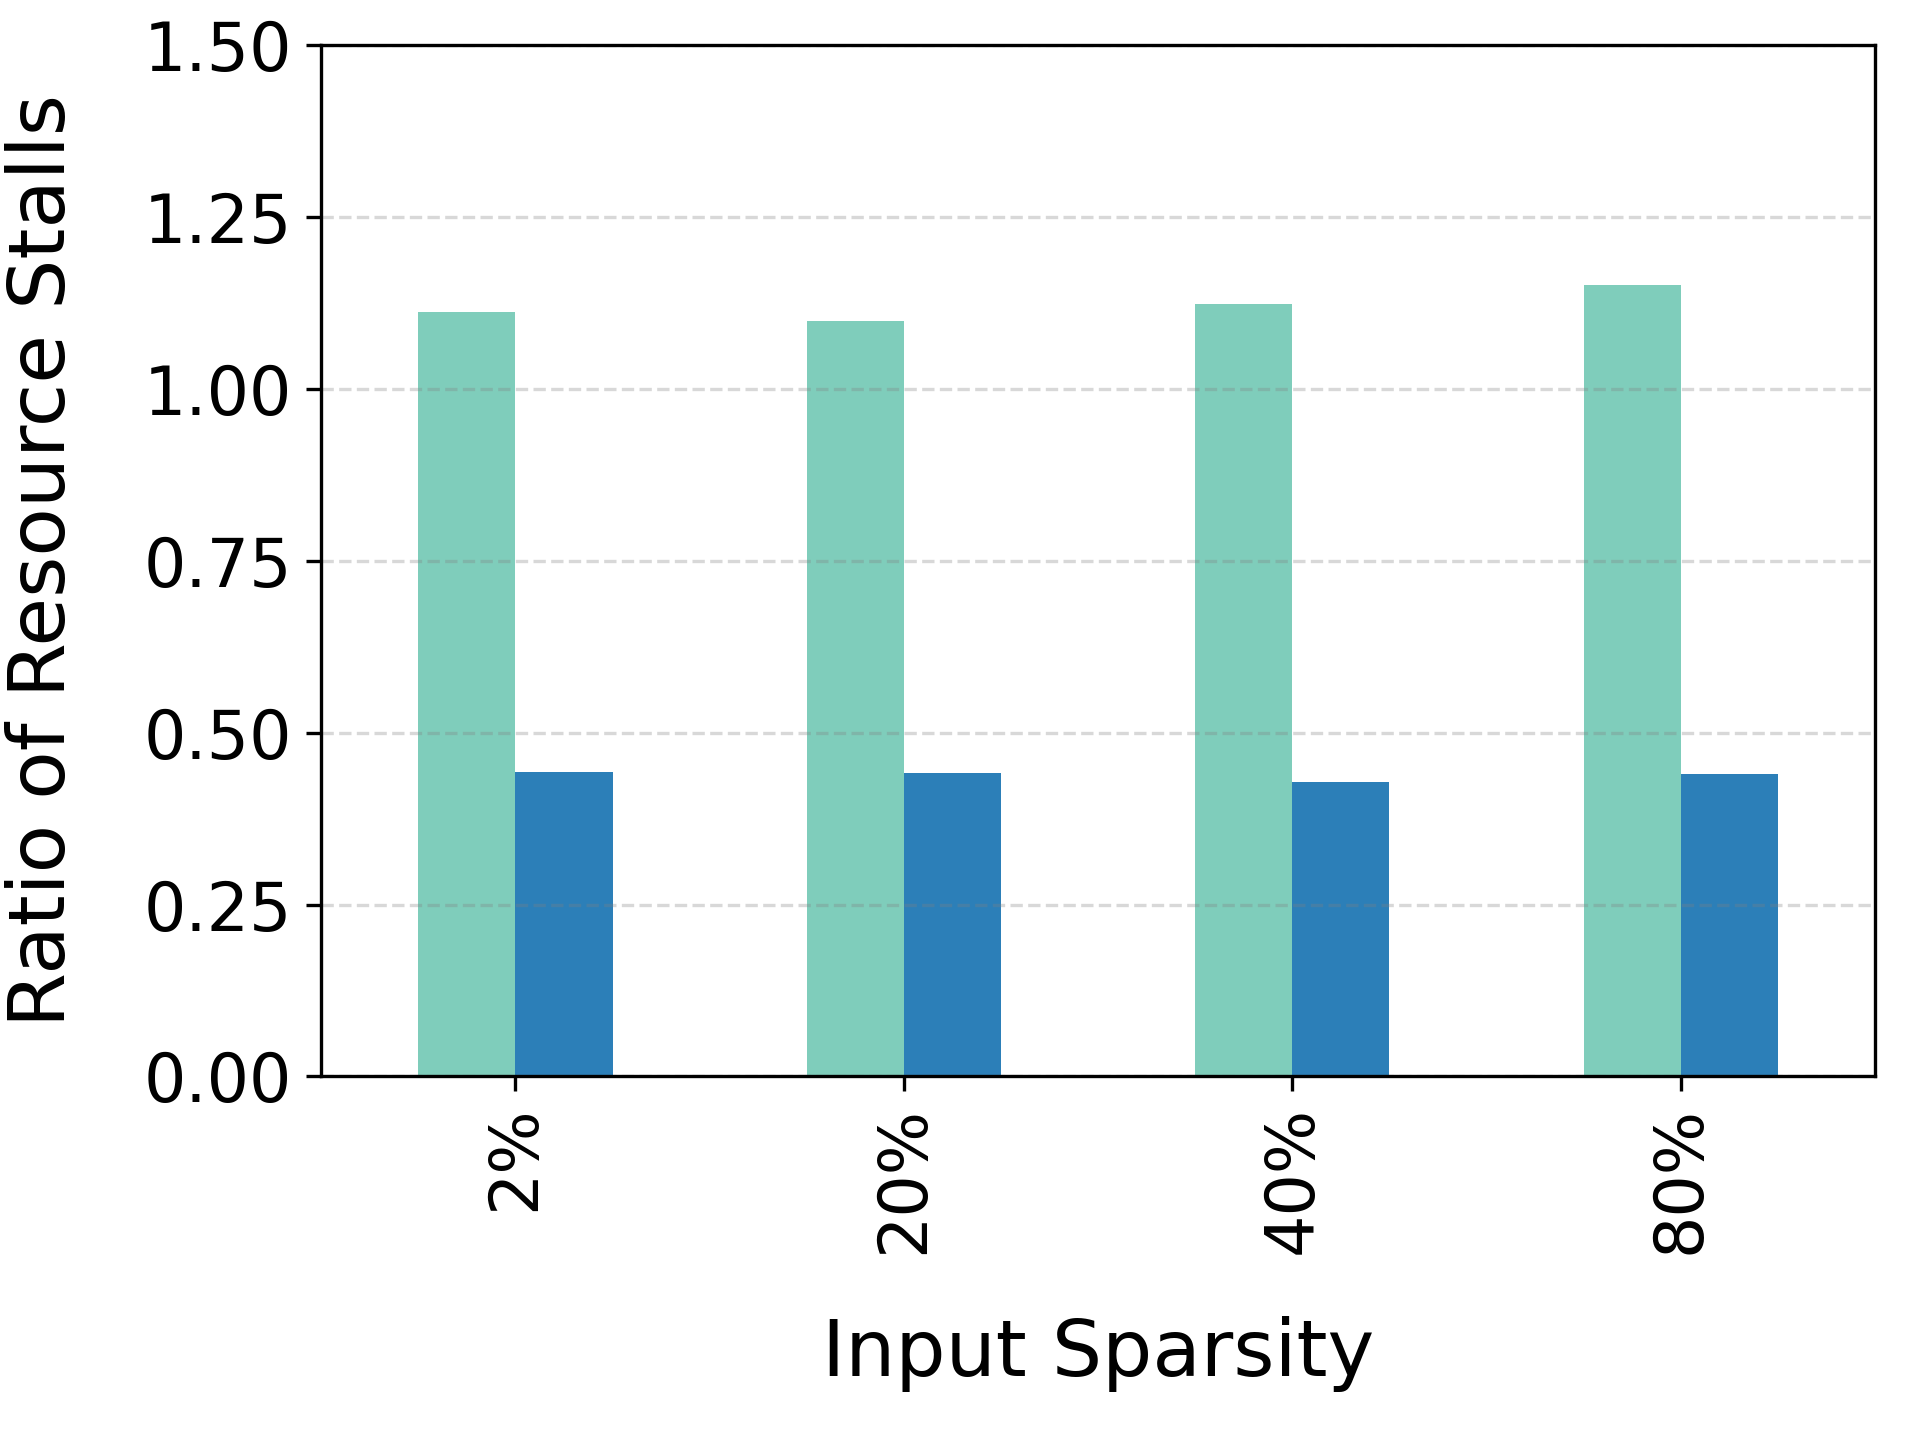
\includegraphics[width=\textwidth]{Figures/Evaluations/if_then_else_few_scatter_resource_stalls.png}
    \caption{Ratio of resource-busy-induced stalls.}
    \label{fig:if-then-else-few-scatter-resource}
  \end{subfigure}%
  \begin{subfigure}{.33\textwidth}
        \centering
    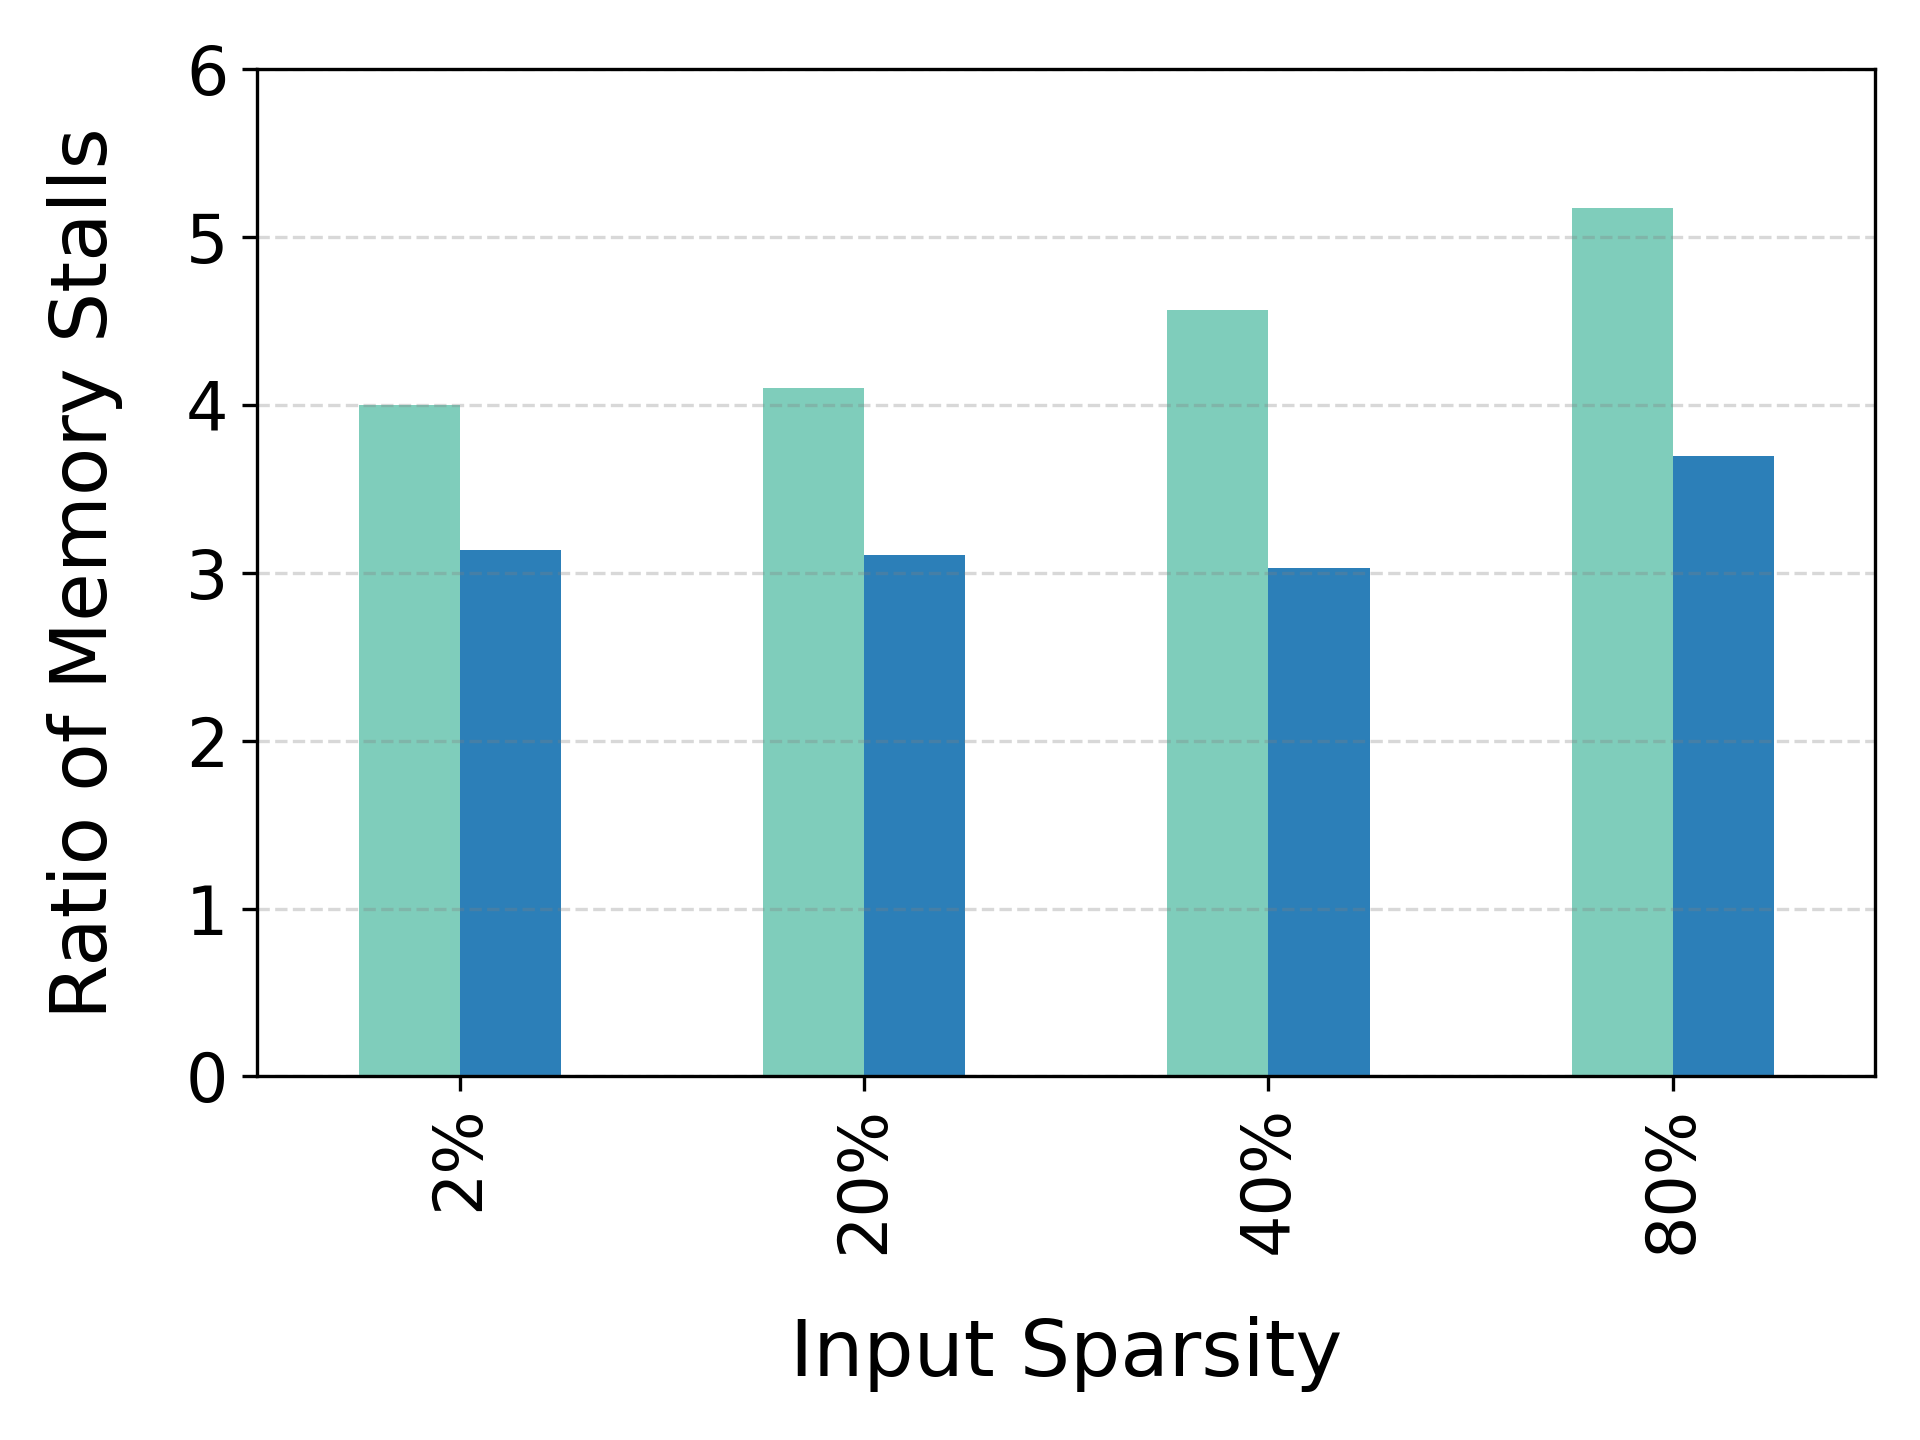
\includegraphics[width=\textwidth]{Figures/Evaluations/if_then_else_few_scatter_mem_stalls.png}
    \caption{Ratio of memory-induced stalls.}
    \label{fig:if-then-else-few-scatter-mem-stalls}
  \end{subfigure}%
  \caption{Evaluation of the \ifElseBench micro-benchmark modified to have fewer store instructions. All metrics are normalized with respect to \ifconverted code (\ifconv).}
\end{figure*}


\begin{figure*}[t]
  \centering
  \begin{subfigure}{4cm}
    \centering
    
\includegraphics[width=\textwidth]{Figures/Evaluations/Legend.png}
  \end{subfigure}\\
  \begin{subfigure}{.33\textwidth}
        \centering
    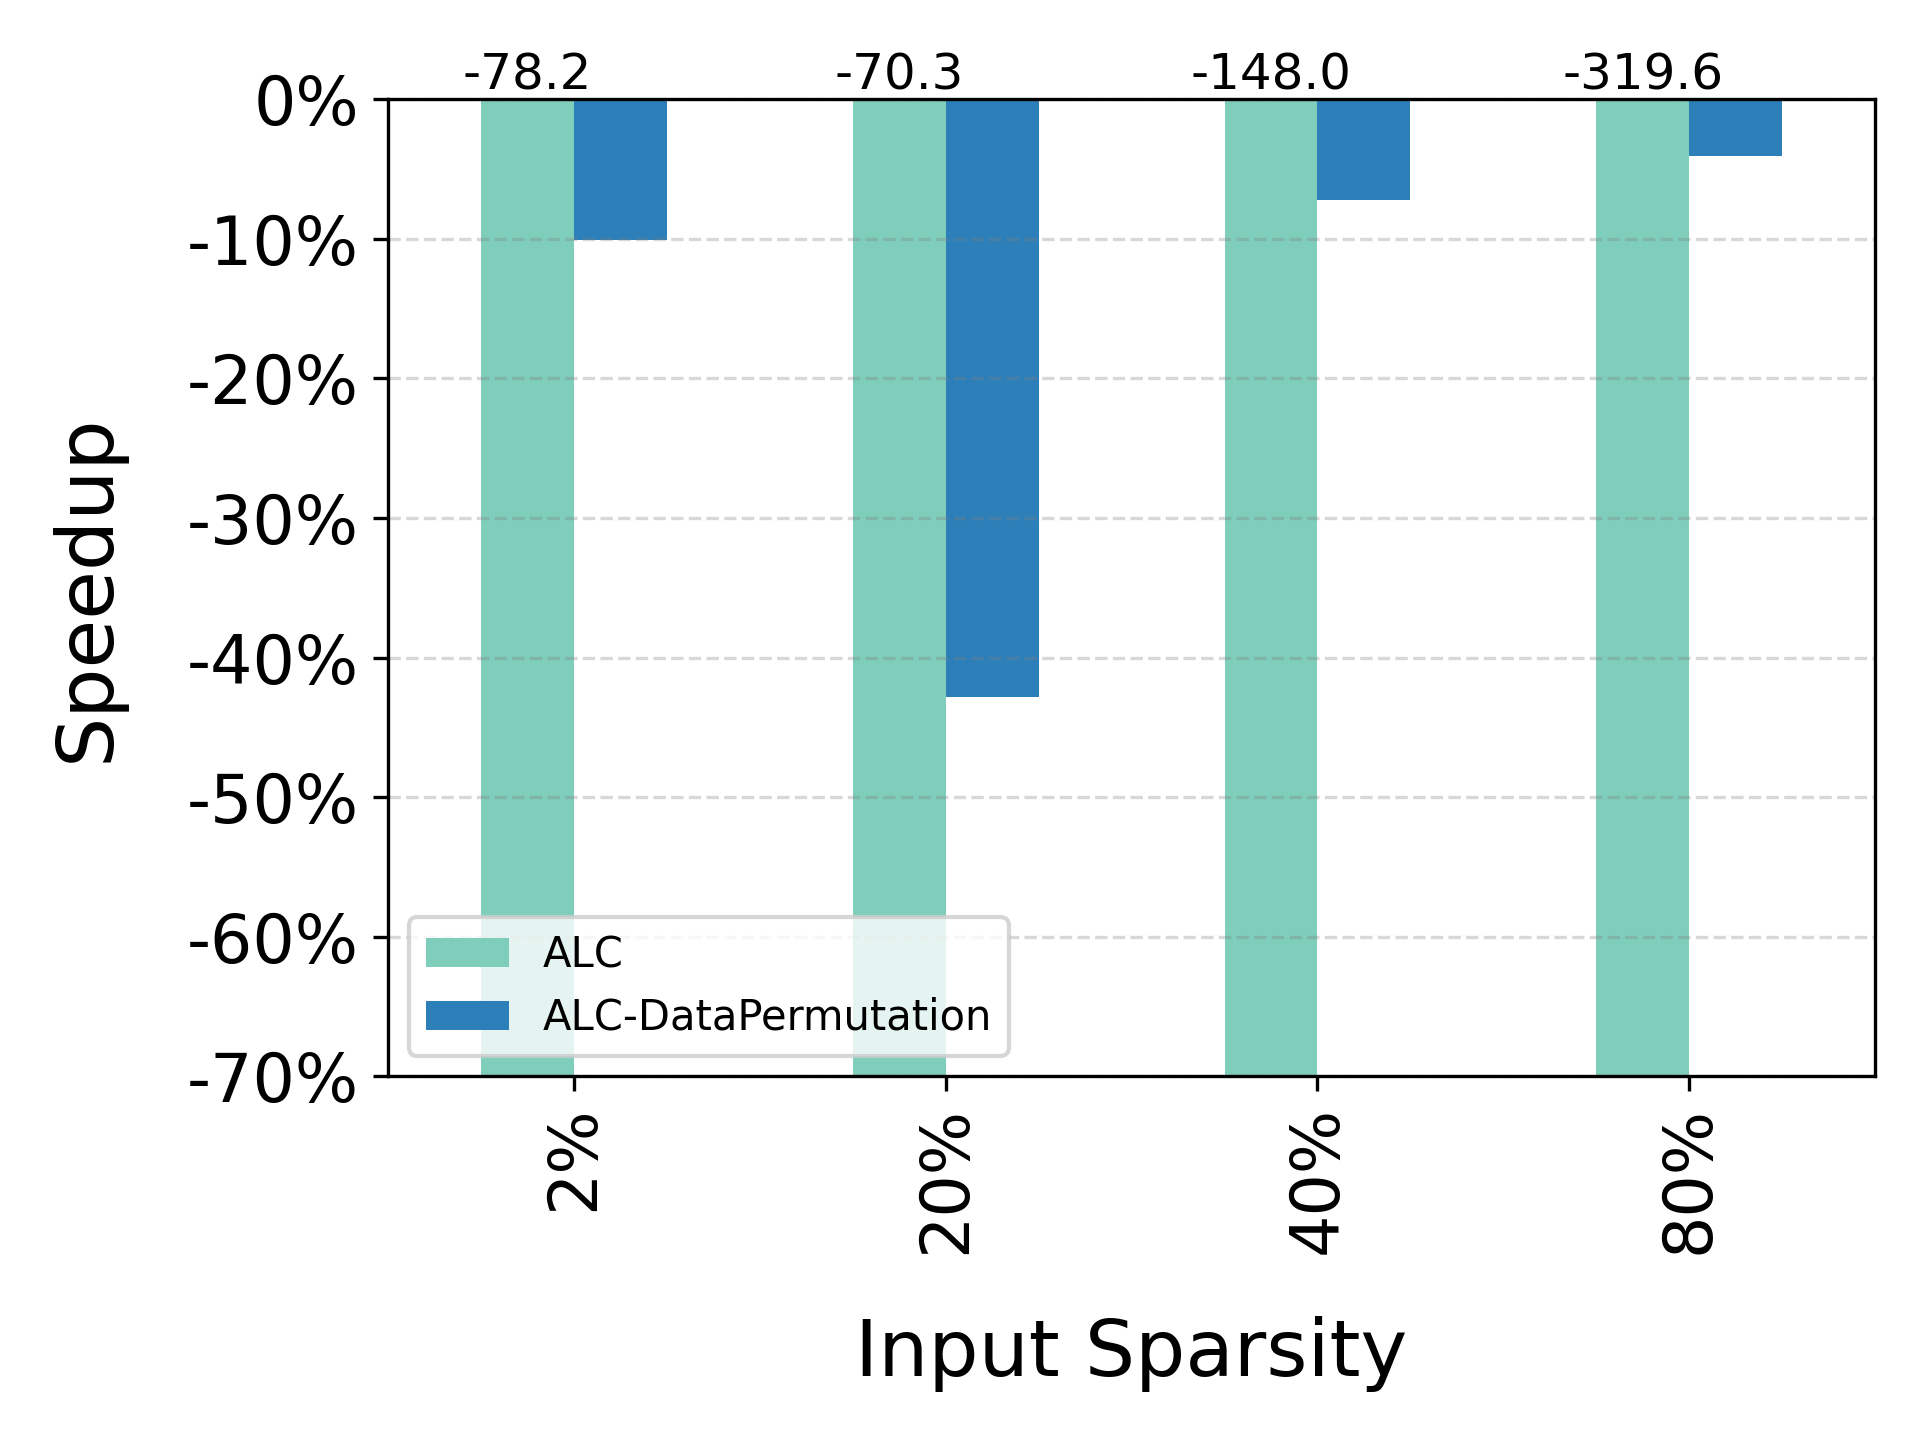
\includegraphics[width=\textwidth]{Figures/Evaluations/single_if_many_scatter_speedup.png}
    \caption{Speedup over \ifconv.}
    \label{fig:single-if-many-scatter}
  \end{subfigure}%
  \begin{subfigure}{.33\textwidth}
        \centering
    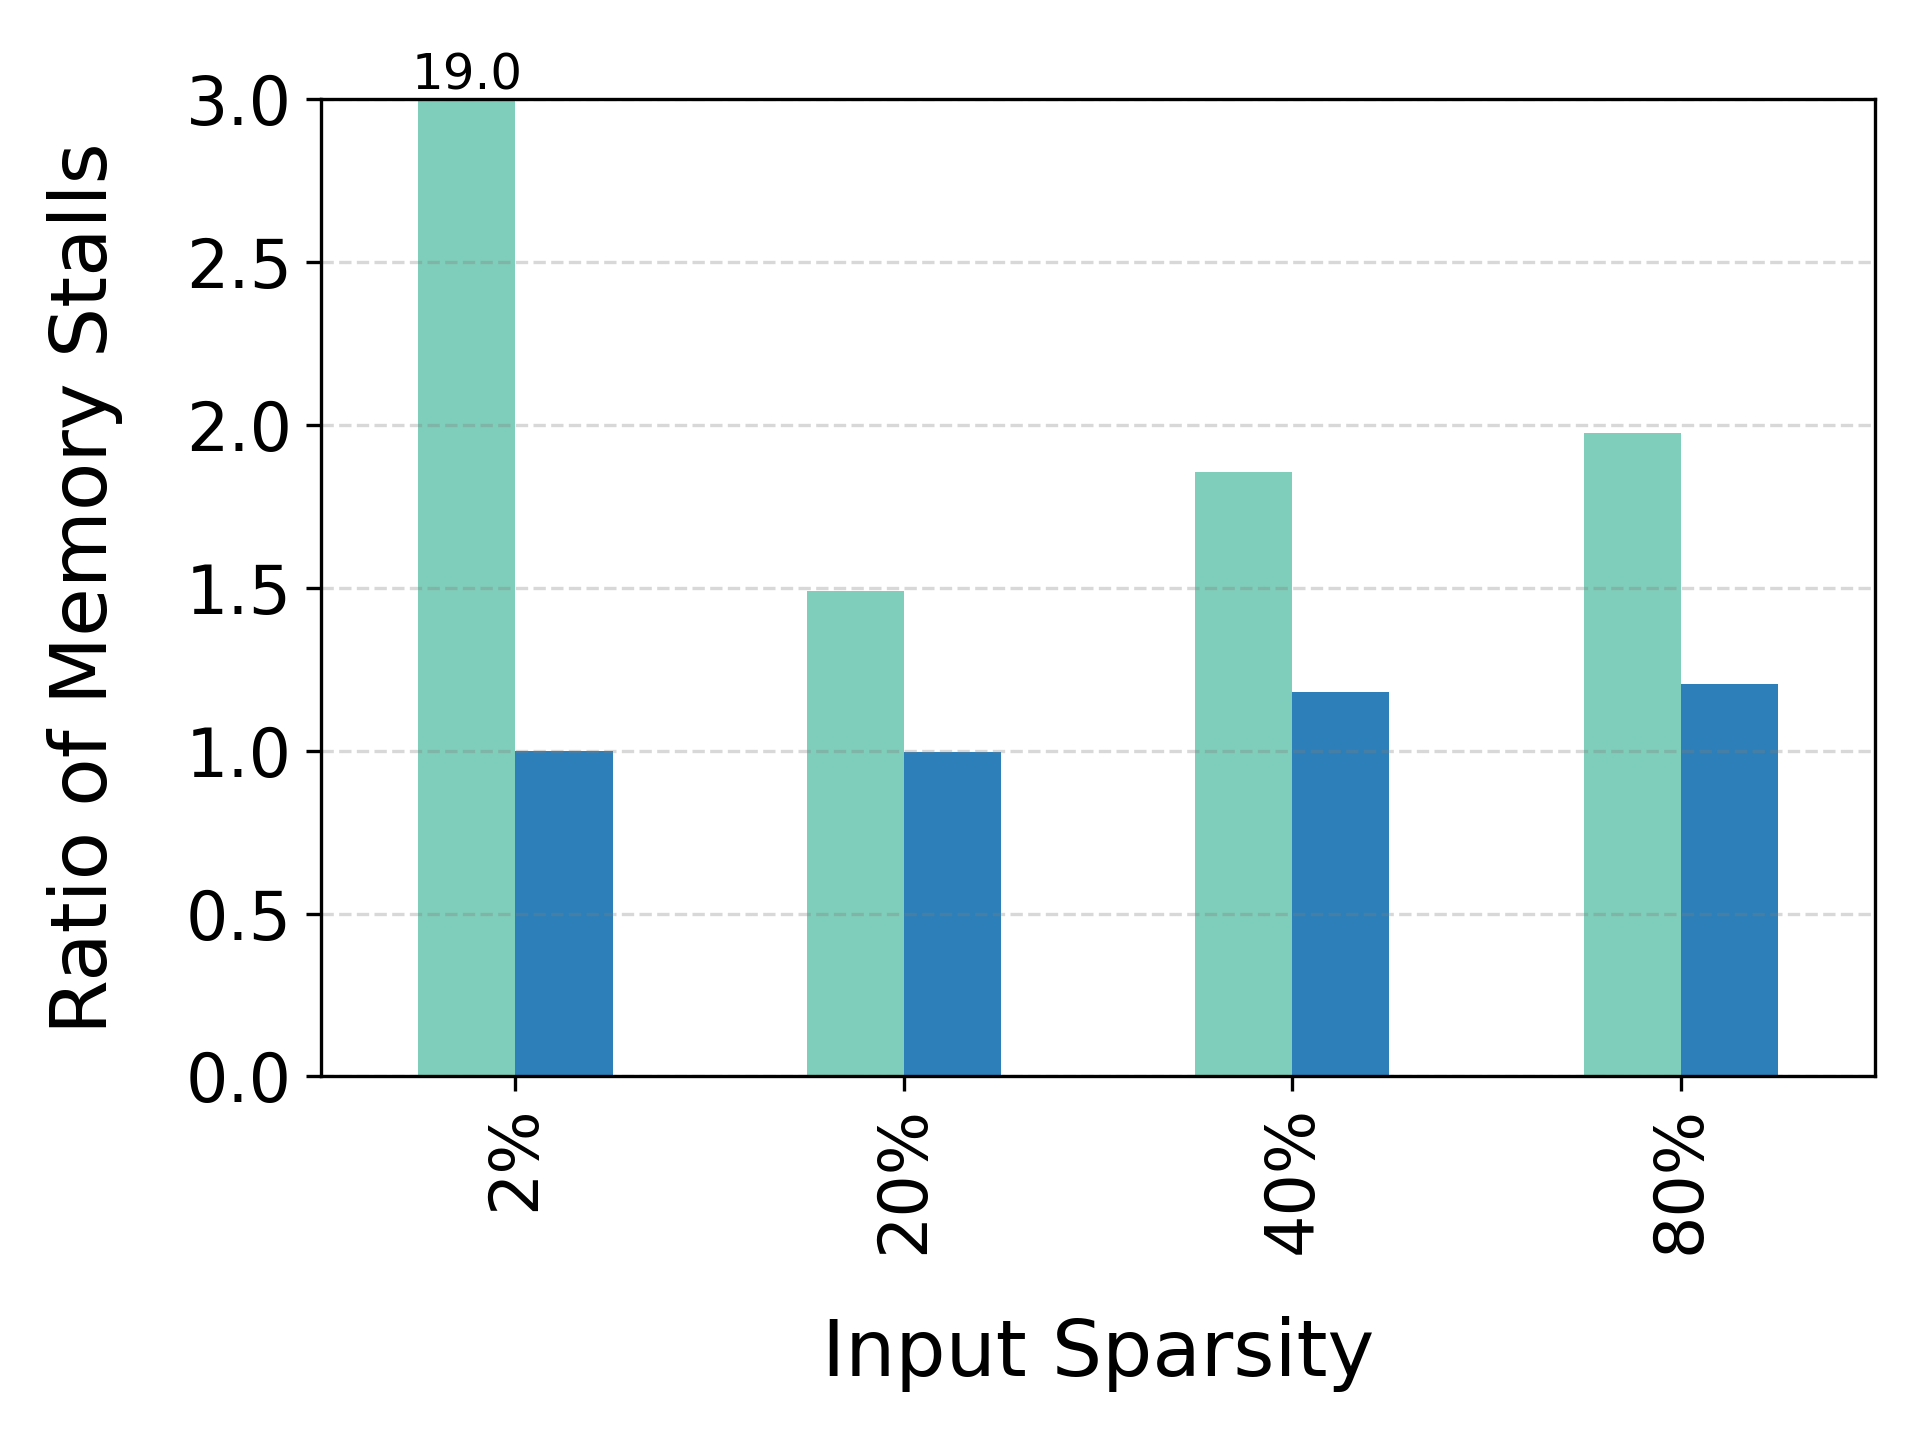
\includegraphics[width=\textwidth]{Figures/Evaluations/single_if_many_scatter_mem_stalls.png}
    \caption{Ratio of memory-induced stalls.}
    \label{fig:single-if-many-scatter-mem-stalls}
  \end{subfigure}
    \begin{subfigure}{.33\textwidth}
        \centering
    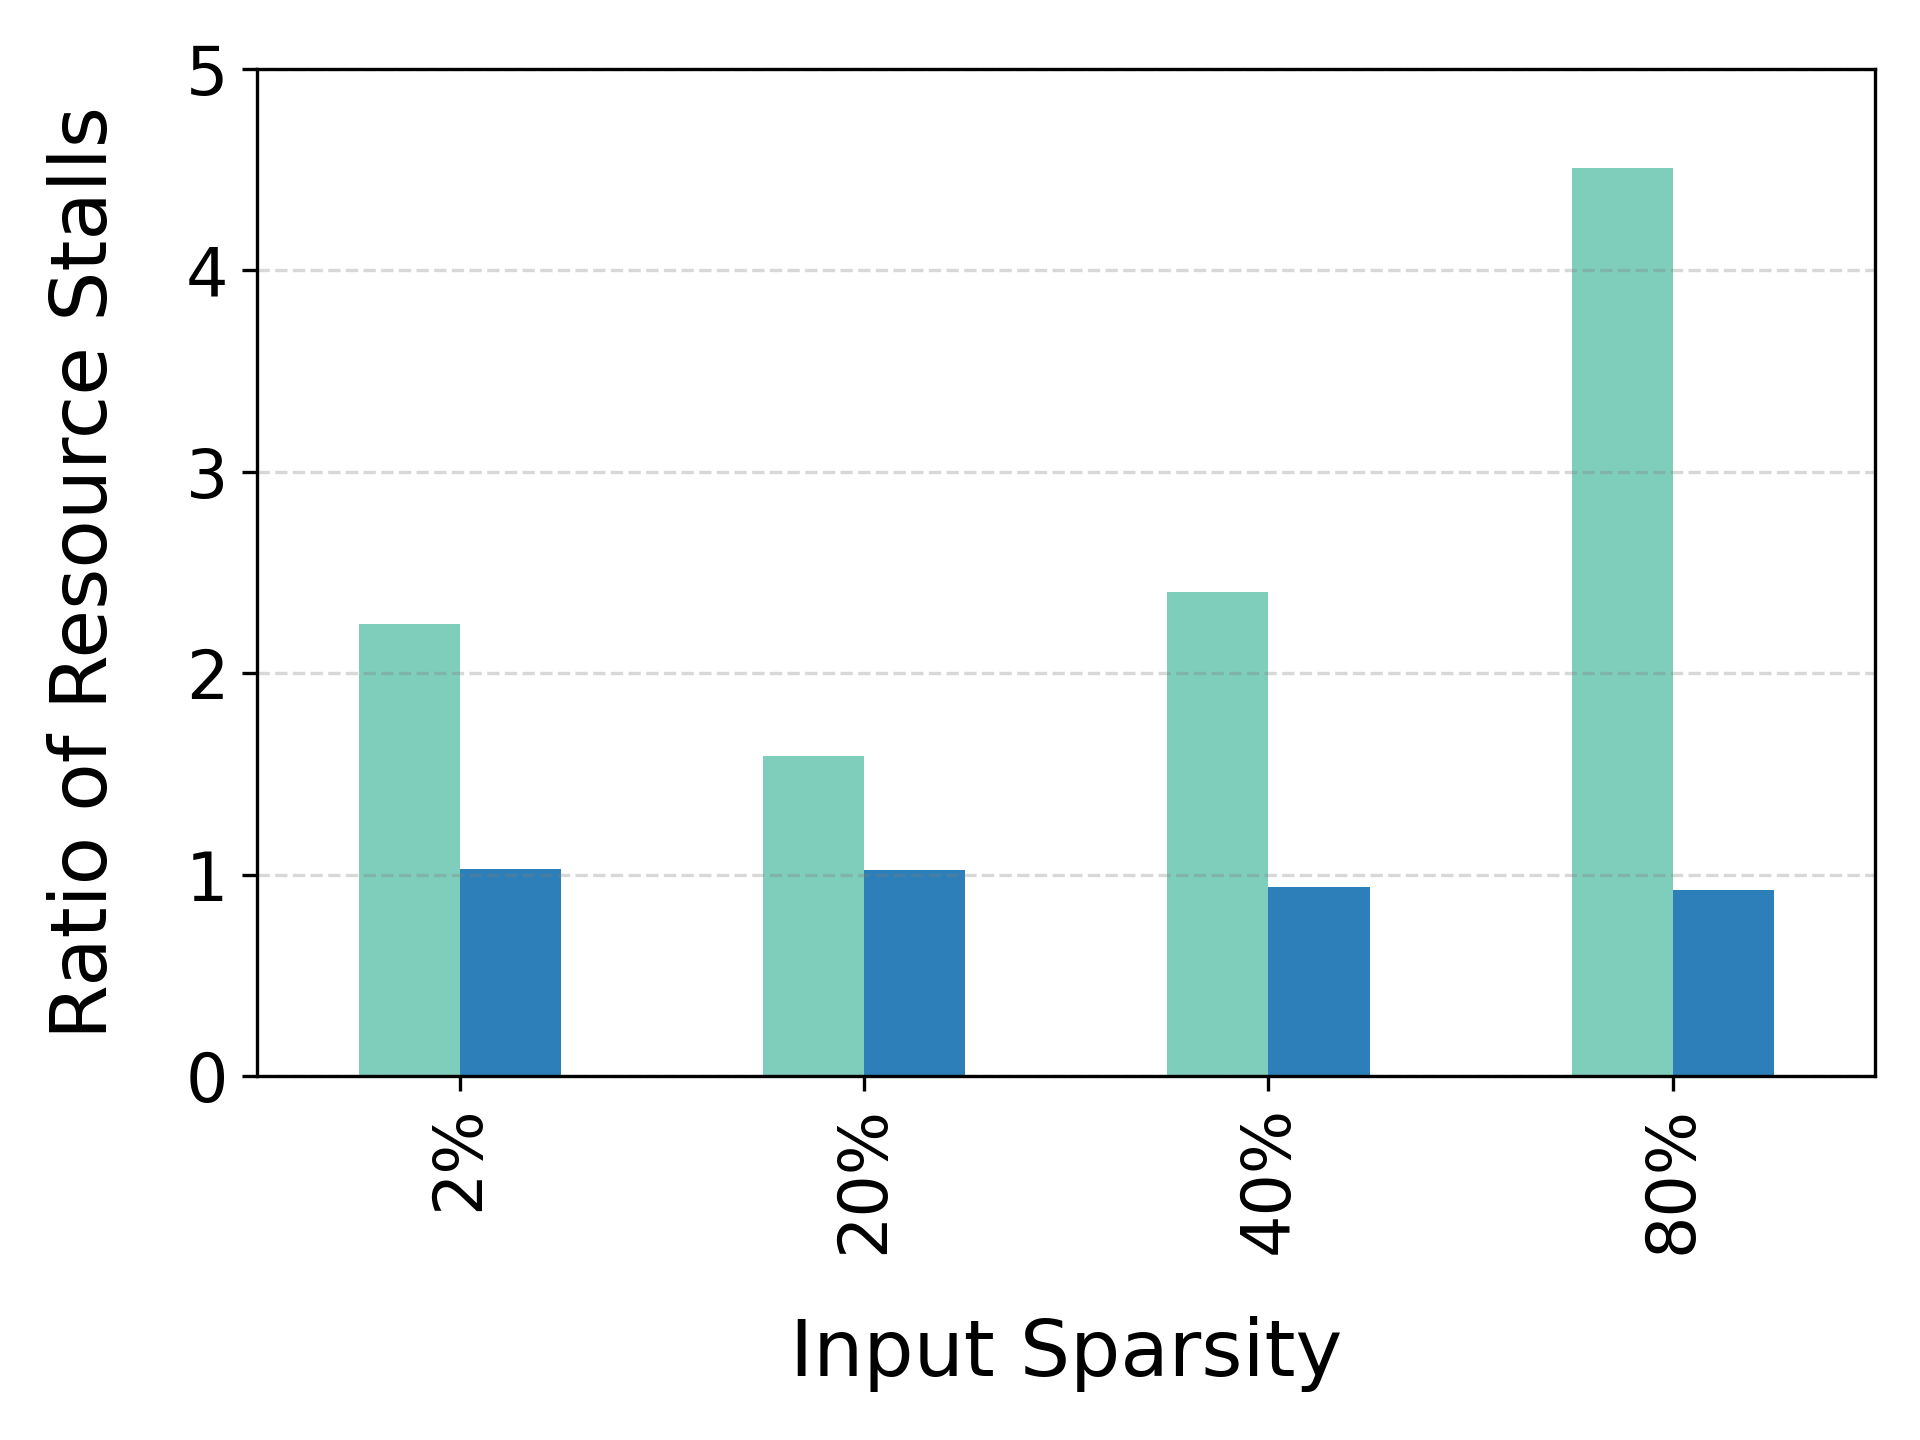
\includegraphics[width=\textwidth]{Figures/Evaluations/single_if_many_scatter_resource_stalls.png}
    \caption{Ratio of resource-busy-induced stalls.}
    \label{fig:single-if-many-scatter-resource-stalls}
  \end{subfigure}
  
  \caption{Performance metrics for each version of the \ifThenBench micro-benchmark that has a single CFDPs. All metrics are normalized with respect to \ifconverted code (\ifconv).}
  \label{fig:single-if-many-scatter}
\end{figure*}

\begin{figure*}[t]
  \centering
  % \begin{subfigure}{4cm}
  %   \centering
  %   
\includegraphics[width=\textwidth]{Figures/Evaluations/Legend.png}
  % \end{subfigure}\\
  \begin{subfigure}{.33\textwidth}
        \centering
    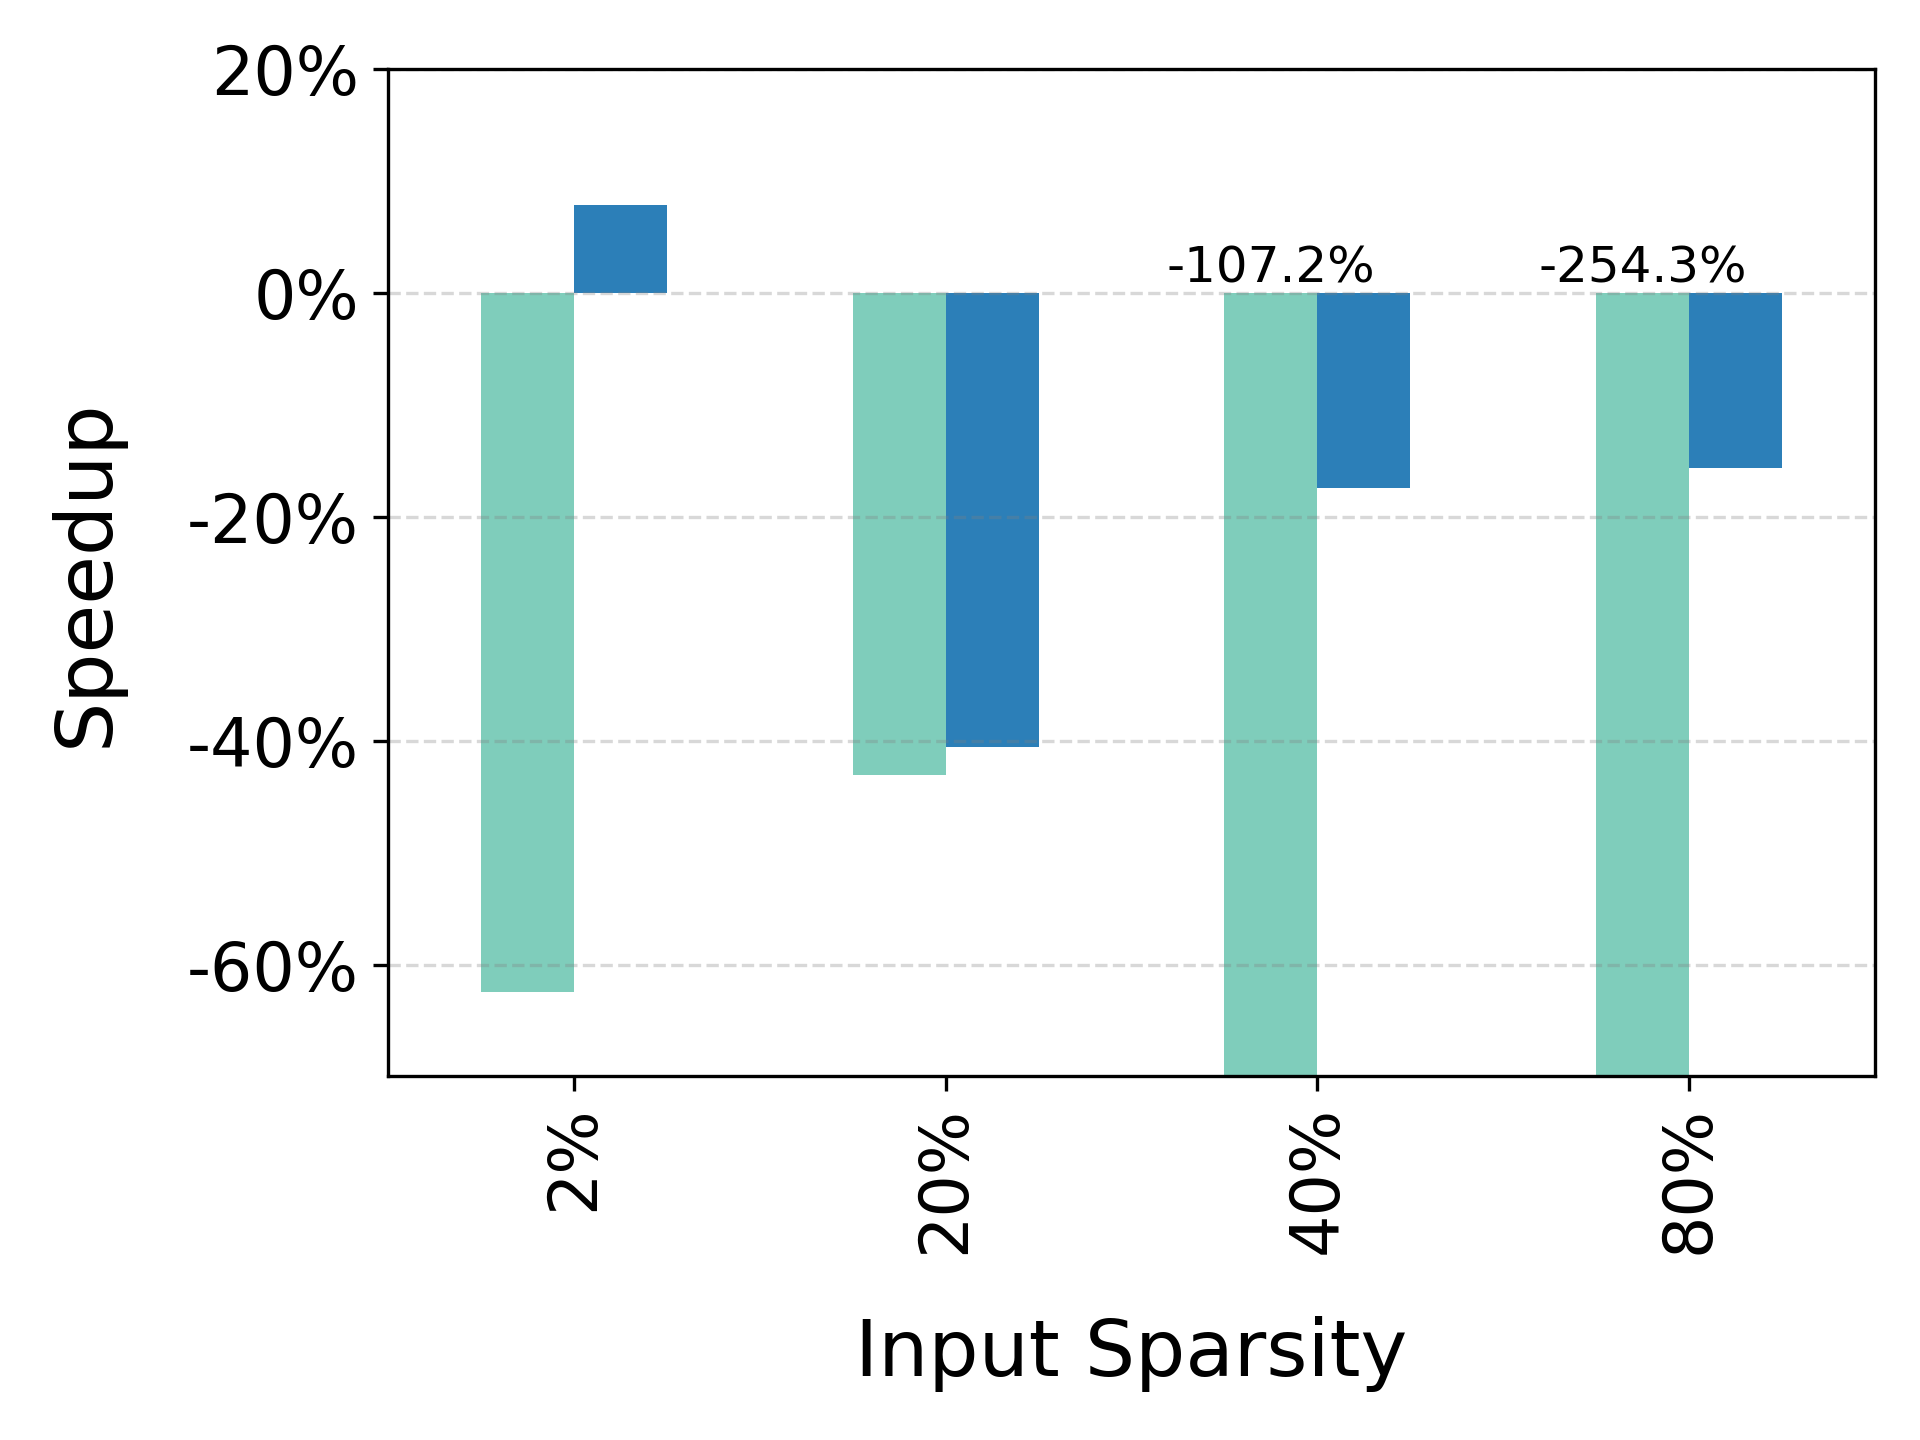
\includegraphics[width=\textwidth]{Figures/Evaluations/single_if_few_scatter_speedup.png}
    \caption{Speedup over \ifconv.}
    \label{fig:single-if-few-scatter-over-ifConv}
  \end{subfigure}%
  \begin{subfigure}{.33\textwidth}
        \centering
    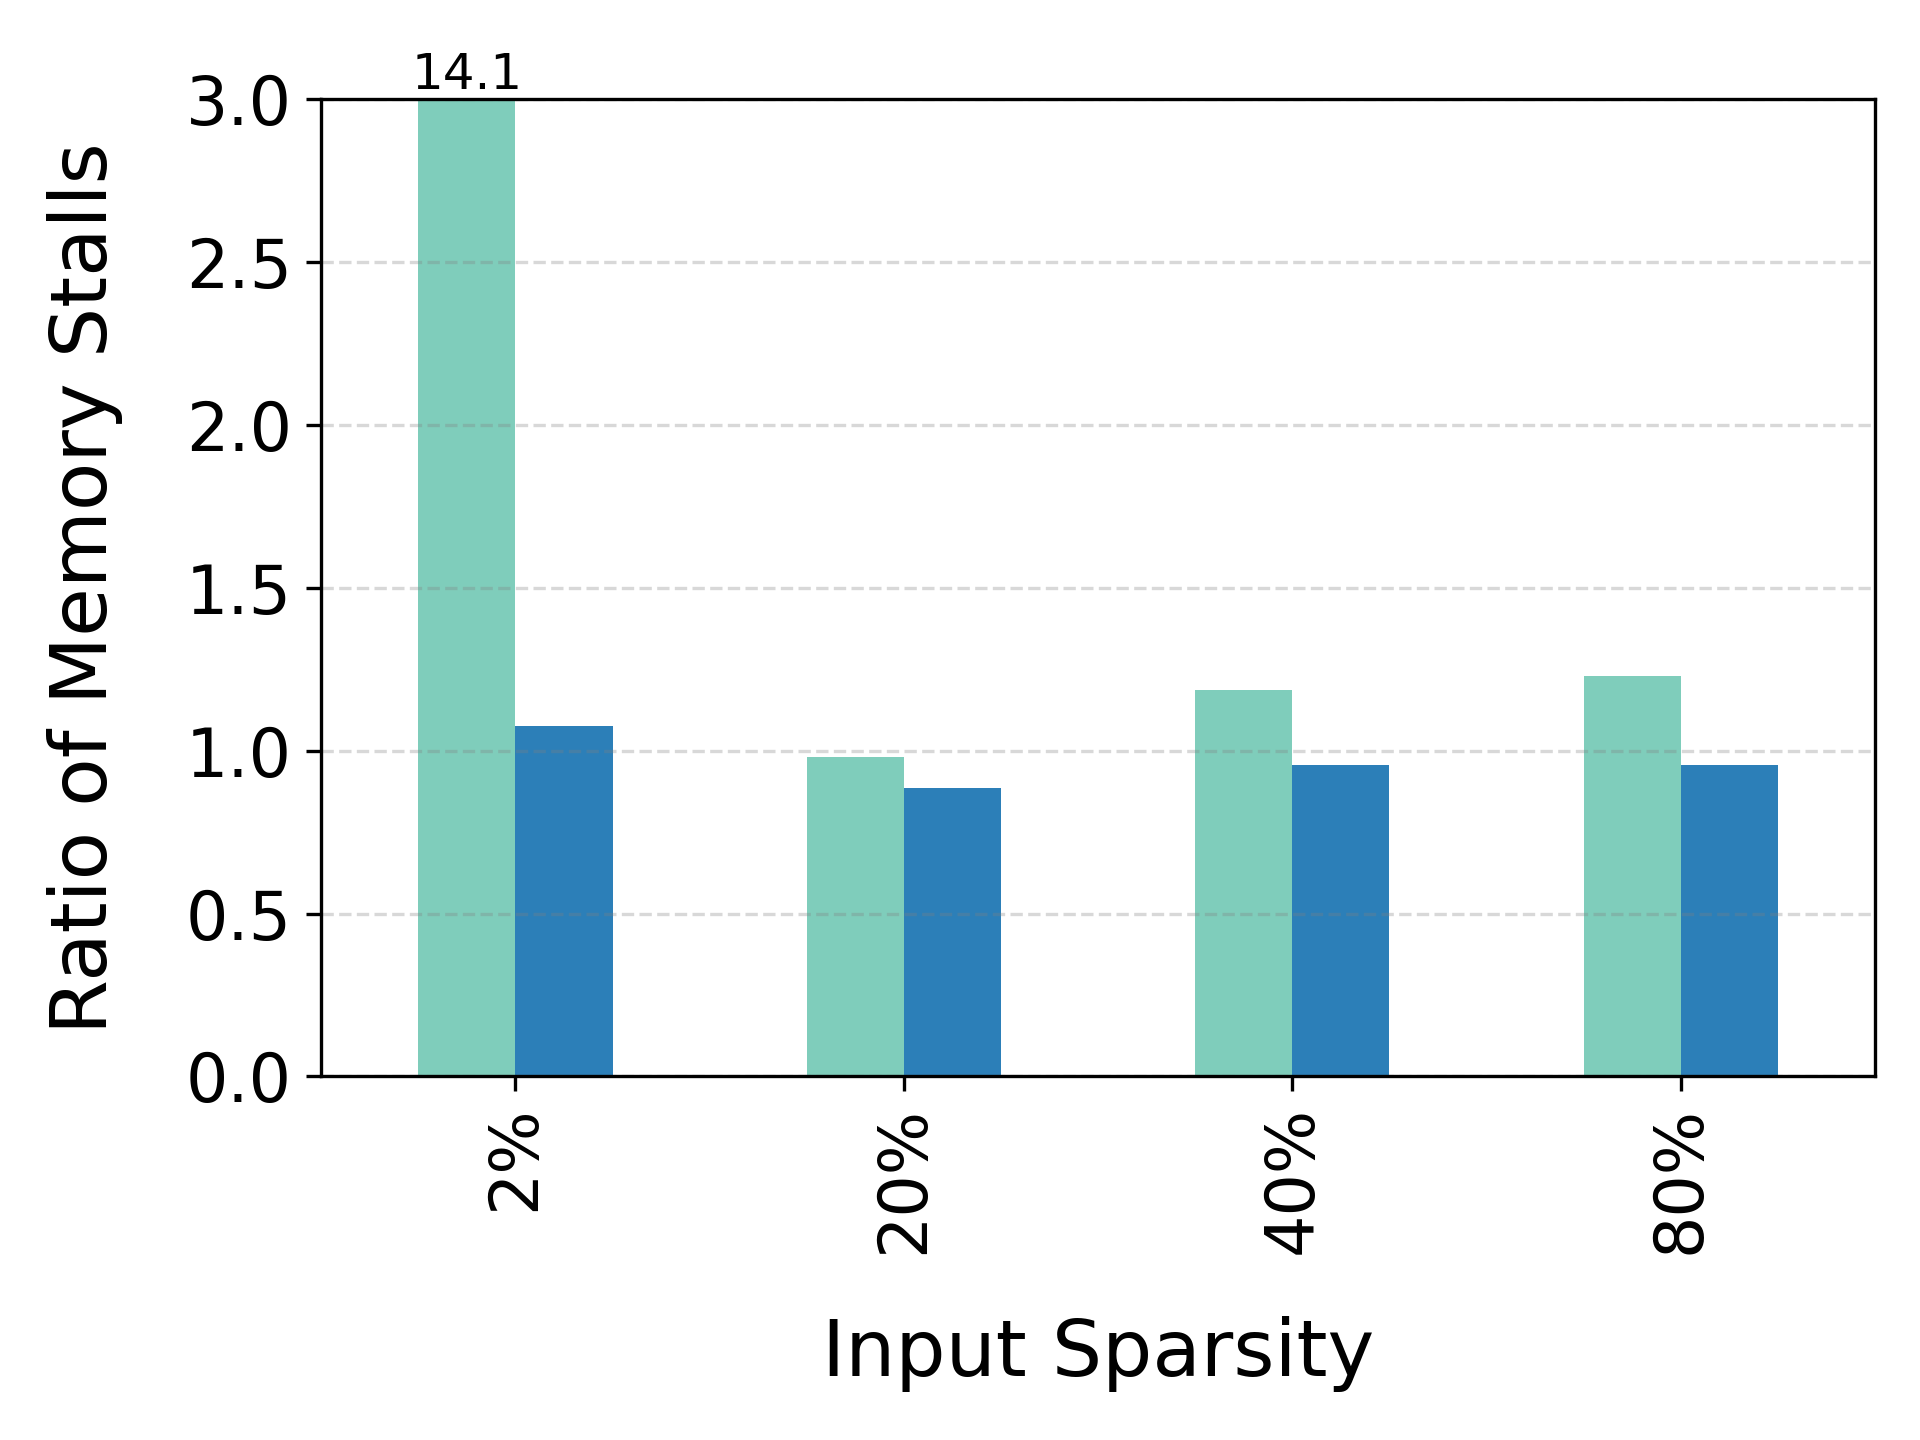
\includegraphics[width=\textwidth]{Figures/Evaluations/single_if_few_scatter_mem_stalls.png}
    \caption{Ratio of memory-induced stalls.}
    \label{fig:single-if-few-scatter-mem-stalls}
  \end{subfigure}
    \begin{subfigure}{.33\textwidth}
        \centering
    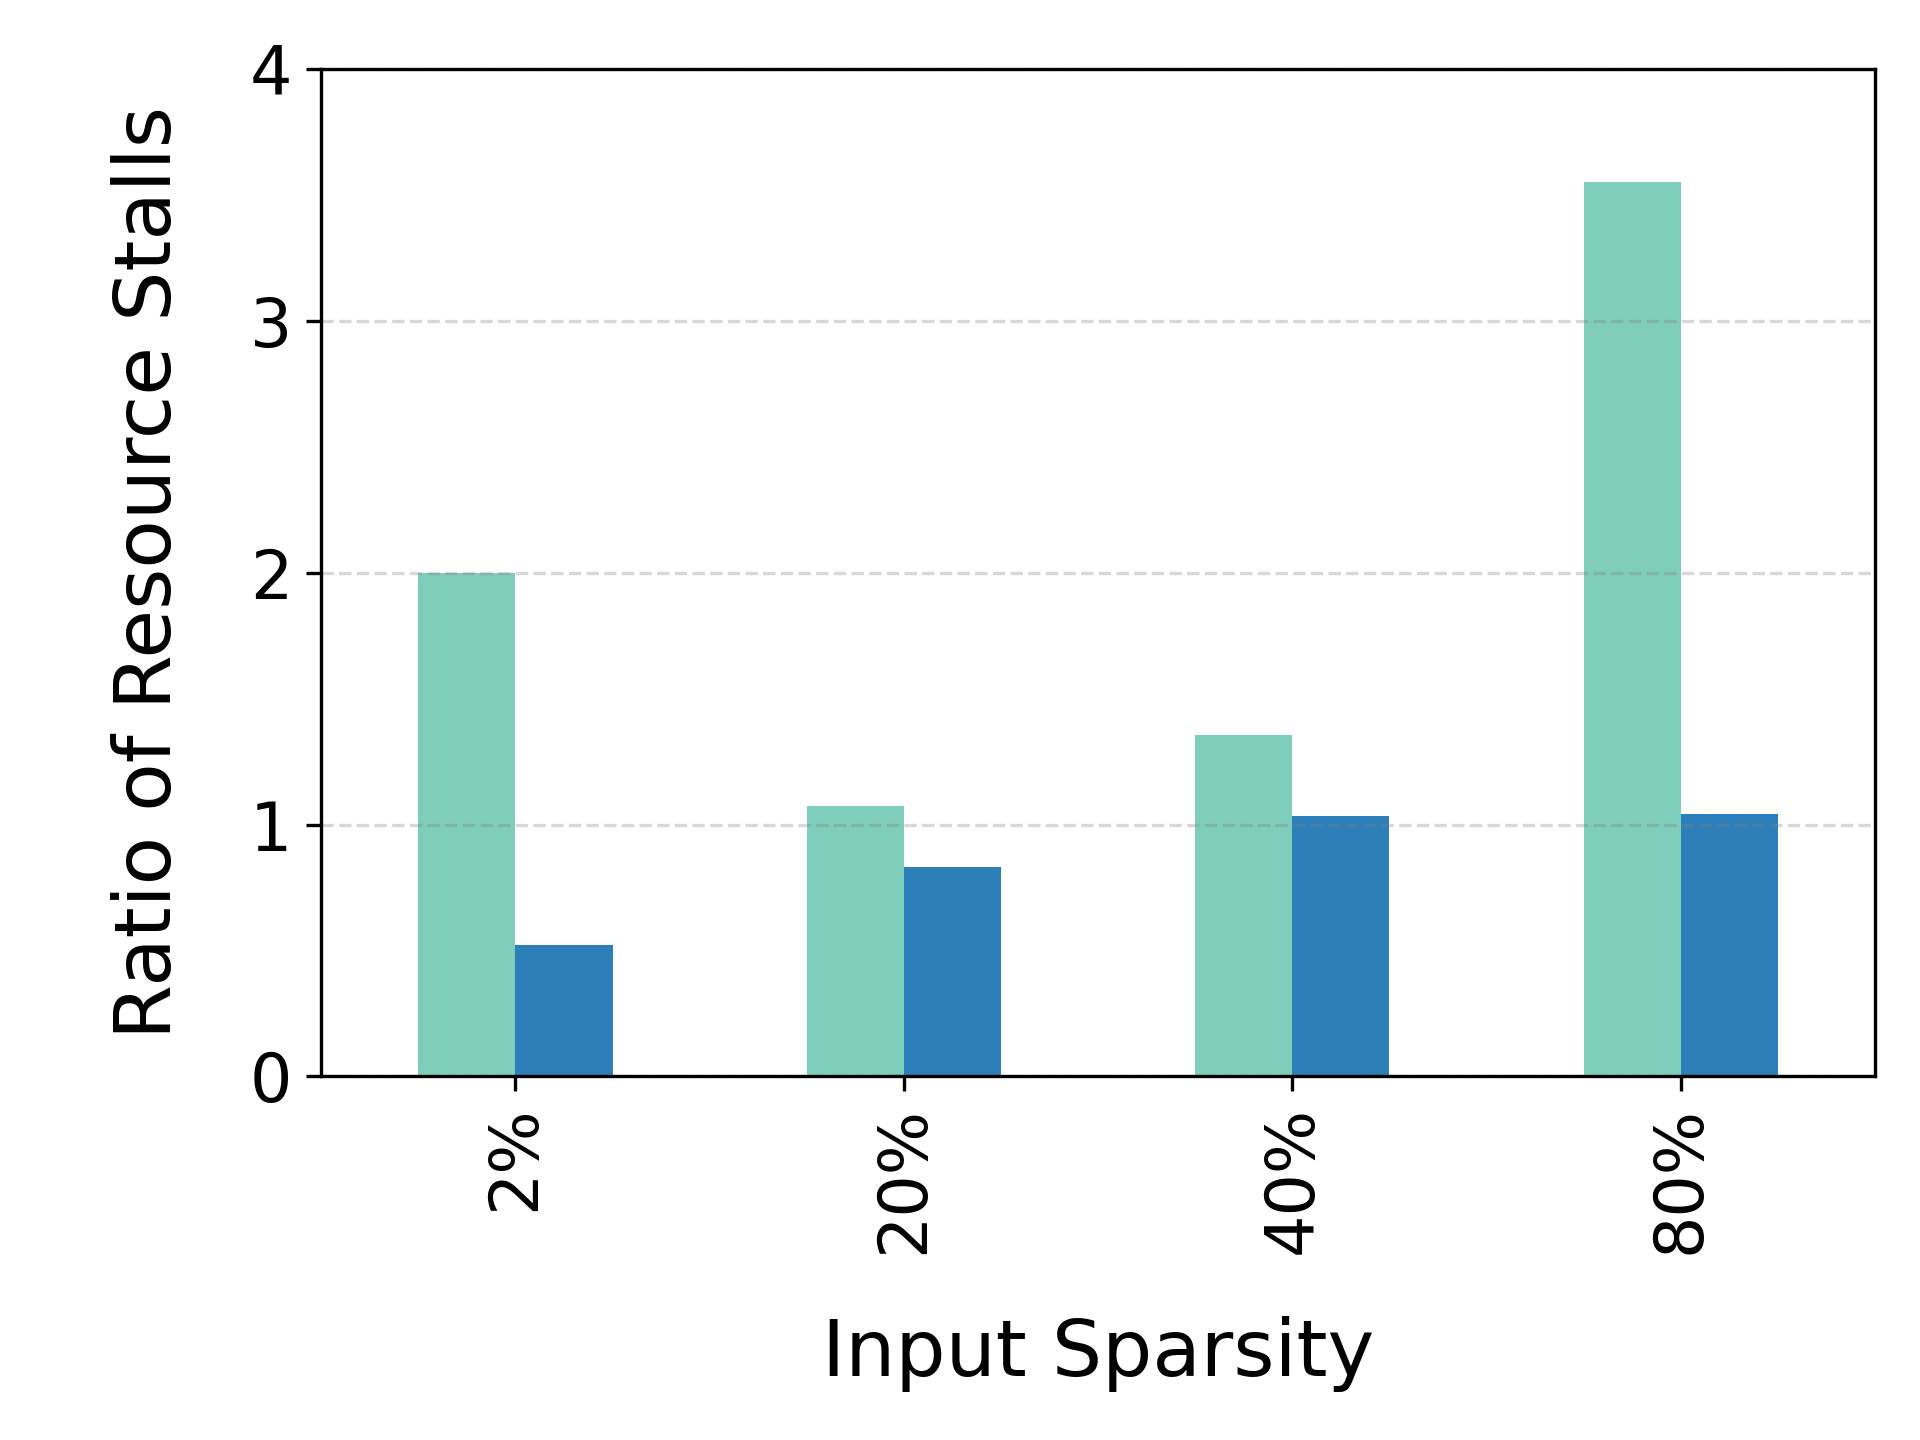
\includegraphics[width=\textwidth]{Figures/Evaluations/single_if_few_scatter_resource_stalls.png}
    \caption{Ratio of resource-busy-induced stalls.}
    \label{fig:single-if-few-scatter-resource-stalls}
  \end{subfigure}
  
  \caption{Performance metrics for each version of the \ifThenBench micro-benchmark modified to have fewer store instructions. All metrics are normalized with respect to \ifconverted code (\ifconv).}
  \label{fig:single-if-few-scatter}
\end{figure*}

\subsection{Data Permutation: More Instructions But Better Performance}
\label{sec:data-permutation-evaluation}

This experiment aims to answer \circled{1} by comparing the performance of each version of the \ifElseBench micro-benchmark generated by Clang.
\rfig{if-then-else-many-scatter-speedup} shows the speedup over \ifconv.
As discussed in \rsec{gathers-scatters-are-bad}, gather instructions have higher latency than regular vector loads, thus hurting \ALC's performance in comparison to \ifconv, which only uses regular vector load instructions.
Such overhead is quantified in \rfig{if-then-else-many-scatter-mem-stalls}, which indicates that the ratio of stalls due to pending memory operations (w.r.t \ifconv) is significantly higher in \ALC than in \ALCdp, which explains \ALCdp better performance.
Also, the address calculations of gather/scatter instructions are executed in the vector units and thus compete for resources and stall other arithmetic operations in \ifElseBench.
As \rfig{if-then-else-many-scatter-resource} indicates, \ALC has more stalls waiting for resources than the baseline \ifconv while \ALCdp has fewer resource stalls than \ALC because gather instructions are eliminated via data permutation.
In addition, \ALCdp outperforms \ifconv for all input sparsity cases and, in particular, by more than $7\%$ in the $80\%$ sparsity case --- a positive answer to question \circled{1}.
\ALCdp performs better than \ifconv even though it executes more instructions to perform data permutation,  as \rfig{if-then-else-many-scatter-inst} indicates.
These data-permutation instructions are vector-to-vector instructions that incur much lower latency than gather instructions do.
\ALCdp still suffers more memory stalls than the baseline \ifconv because of the high latency of scatter stores that, usually, cannot be avoided.
In contrast,  \ALC always performs worse than \ifconv and shows performance degradation of up to $6\%$ in the $40\%$ sparsity case.

\subsection{Scatter Instructions Significantly Impact Performance}
\label{sec:eval-scatters-costs}

In this experiment, the code of the \ifElseBench micro-benchmark is modified to have fewer stores --- only one per \cpath ---, but it has the same number of arithmetic and load operations.
Fewer store operations translate to fewer scatter instructions in the compiler-generated ALC code.
Therefore, an increase in ALC's performance with fewer scatter operations indicates a positive answer to \circled{2}.
As \rfig{if-then-else-few-scatter-speedup} indicates, with fewer scatter stores both \ALC and \ALCdp outperform the baseline \ifconv.
Moreover, \ALCdp is four times faster than \ALC, outperforming \ifconv by up to $79\%$ in the $2\%$ sparsity case, a strong indicator of the effectiveness of eliminating both predicated instructions and gather loads.
\rfig{if-then-else-few-scatter-resource} shows a significant reduction in the number of resource stalls for \ALCdp as a direct result of having fewer scatter store instructions and thus explains the speedup over \ifconv.
Stalls due to memory operations follow the same trend as in the \ifElseBench micro-benchmark, as indicated in \rfig{if-then-else-few-scatter-mem-stalls}, evidence that arithmetic operations can amortize the effects of memory stalls.
Still, address calculations for gather/scatter instructions compete for resources resulting in a significant number of resource-busy stalls. 

\subsection{Data Permutation Improves ALC}
\label{sec:eval-single-if}

This experiment evaluates the ALC algorithm modification discussed in \rsec{single-if-statement-approach} on the \ifThenBench micro-benchmark.
\rfig{single-if-many-scatter} presents speedups of \ALC and \ALCdp over \ifconv.
In this case, both ALC versions are unable to provide improvements over \ifconv and result in performance degradation.
The single control-flow data path case is challenging for any variant of ALC because, unlike the \ifElseBench case that has two \cpaths, considerably fewer instructions are executed with inactive lanes.
The results indicate a negative answer to \circled{3}, \ie, in general, it is not beneficial to apply ALC on loops with a single \cpath.
Nevertheless, \ALCdp provides significant speedup over \ALC by eliminating gather load instructions.
Moreover, and similar to the two \cpath cases, both memory and resource stalls are lower with \ALCdp than with \ALC, as \rfig{single-if-many-scatter-mem-stalls} and \rfig{single-if-many-scatter-resource-stalls} indicate.
As seen in \rfig{single-if-few-scatter-over-ifConv}, even in a modified version of \ifThenBench with fewer store instructions, neither version of ALC can outperform \ifconv.
The exception is the very sparse case ($2\%$), where \ALCdp provides a speedup of $7\%$ over \ifconv.
Thus, the results indicate that \ALCdp can benefit loops with single \cpath and very few true predicates.
\ifThenBench, which has fewer stores, has similar behavior in terms of resource and memory stalls, as \rfig{single-if-few-scatter-mem-stalls} and \rfig{single-if-few-scatter-resource-stalls} indicate, as the same benchmark with more store instructions.

\subsection{Conditionally Incremented Array Indexes}
\label{sec:eval-limitations}

The ALC analysis pass found many loops in existing benchmarks (e.g. SPEC CPU 2017~\cite{spec} and MiBench~\cite{MiBench}) that could be legally transformed by ALC transformation.
However, the cost/benefit analysis indicated that those loops would not benefit from ALC because they contained not enough instructions to amortize the cost of index and data permutation (see \rsec{alc-analysis}).

Another challenge discovered when trying to apply ALC to existing benchmarks that contain loops with conditional statements, such as the ones in MiBench~\cite{MiBench}, is related to efficient mappings of conditional computations to vector code. 

\begin{center}
\begin{minipage}[t]{0.99\columnwidth}
\begin{lstlisting}[
escapechar=|,
language=C,
caption={Conditional increment of array indexing variable.},
label=lst:cond-indvar]
for (int i = 0, j = 0; i < n; i++) {
    if (cond[i]) { |\label{lst:cond-indvar:cond}|
        b[i] = a[j];
        j++; |\label{lst:cond-indvar:j-inc}|
    }
}
\end{lstlisting} 
\end{minipage}
\end{center}

For example, \rlst{cond-indvar} shows a simplified example of a loop pattern that is widely found in the \code{jpeg} benchmark in MiBench.
The loop index into array \code{a} with variable \code{j}, which is conditionally incremented when (\rline{cond-indvar:j-inc}) \code{cond[i]} is true (\rline{cond-indvar:cond}).
To the best of our knowledge, there is no single instruction in modern vector ISAs that can compute an index vector with the values of \code{j} in this case.
Therefore multiple instructions would be required, which might make it unprofitable to vectorize such loops.
Neither Clang, GCC, nor Arm's Clang vectorized the loops in SPEC CPU 2017 with the pattern shown in \rlst{cond-indvar}.
Because of such non-trivially vectorizable pattern, this work did not find opportunities to apply ALC as a compiler-enabled transformation to these benchmark suites.
If future versions of vector ISAs include instructions to create conditionally-strided index vectors then more loops could become candidates for \ifconversion and ALC.
A potential workaround would be to compute the values of \code{j} on a separate loop, storing such values in a temporary array, and then using the computed array to index \code{a}.
However, hoisting the computation might not always be possible because of intra-iteration dependencies.

\iffalse
% ######  ATTENTION #############
% The text bellow was left as a reference and is not going to be used for the paper.
% ######  ATTENTION #############


%In \rfig{if-then-else-many-scatter-inst} reduction of dynamically executed instructions with respect to scalar code is being demonstrated. \ALC and if-converted code reduce the number of executed instructions by more than 80\% while \ALCdp reduces them by around 75\%. This is because permutation logic includes a considerable number of instructions, and adding it for every load instructions would result in an increase in the number of instructions. However, comparing number of instructions with the speedups confirms that instructions used for permutation are very fast and although \ALCdp executes more instructions, it provides better performance in terms of execution time.

%\rfig{if-then-else-many-scatter-mem-stalls} shows what ratio of cycles the processor is stalled due to memory and. \ifconv has the least number of memory stalls as it only uses regular memory instructions, loading from and storing to consecutive memory addresses. On the other hand, \ALC uses gather loads and scatter stores, causing significant overheads. Using \ALCdp eliminates any gather instructions, which results in fewer memory stalls however, it still uses scatter stores which lead to more stalls than \ifconv.

\begin{figure*}[t]
  \centering
  \begin{subfigure}{5cm}
    \centering
    
\includegraphics[width=\textwidth]{Figures/Evaluations/Legend.png}
  \end{subfigure}\\
  \begin{subfigure}{.499\textwidth}
    \centering
    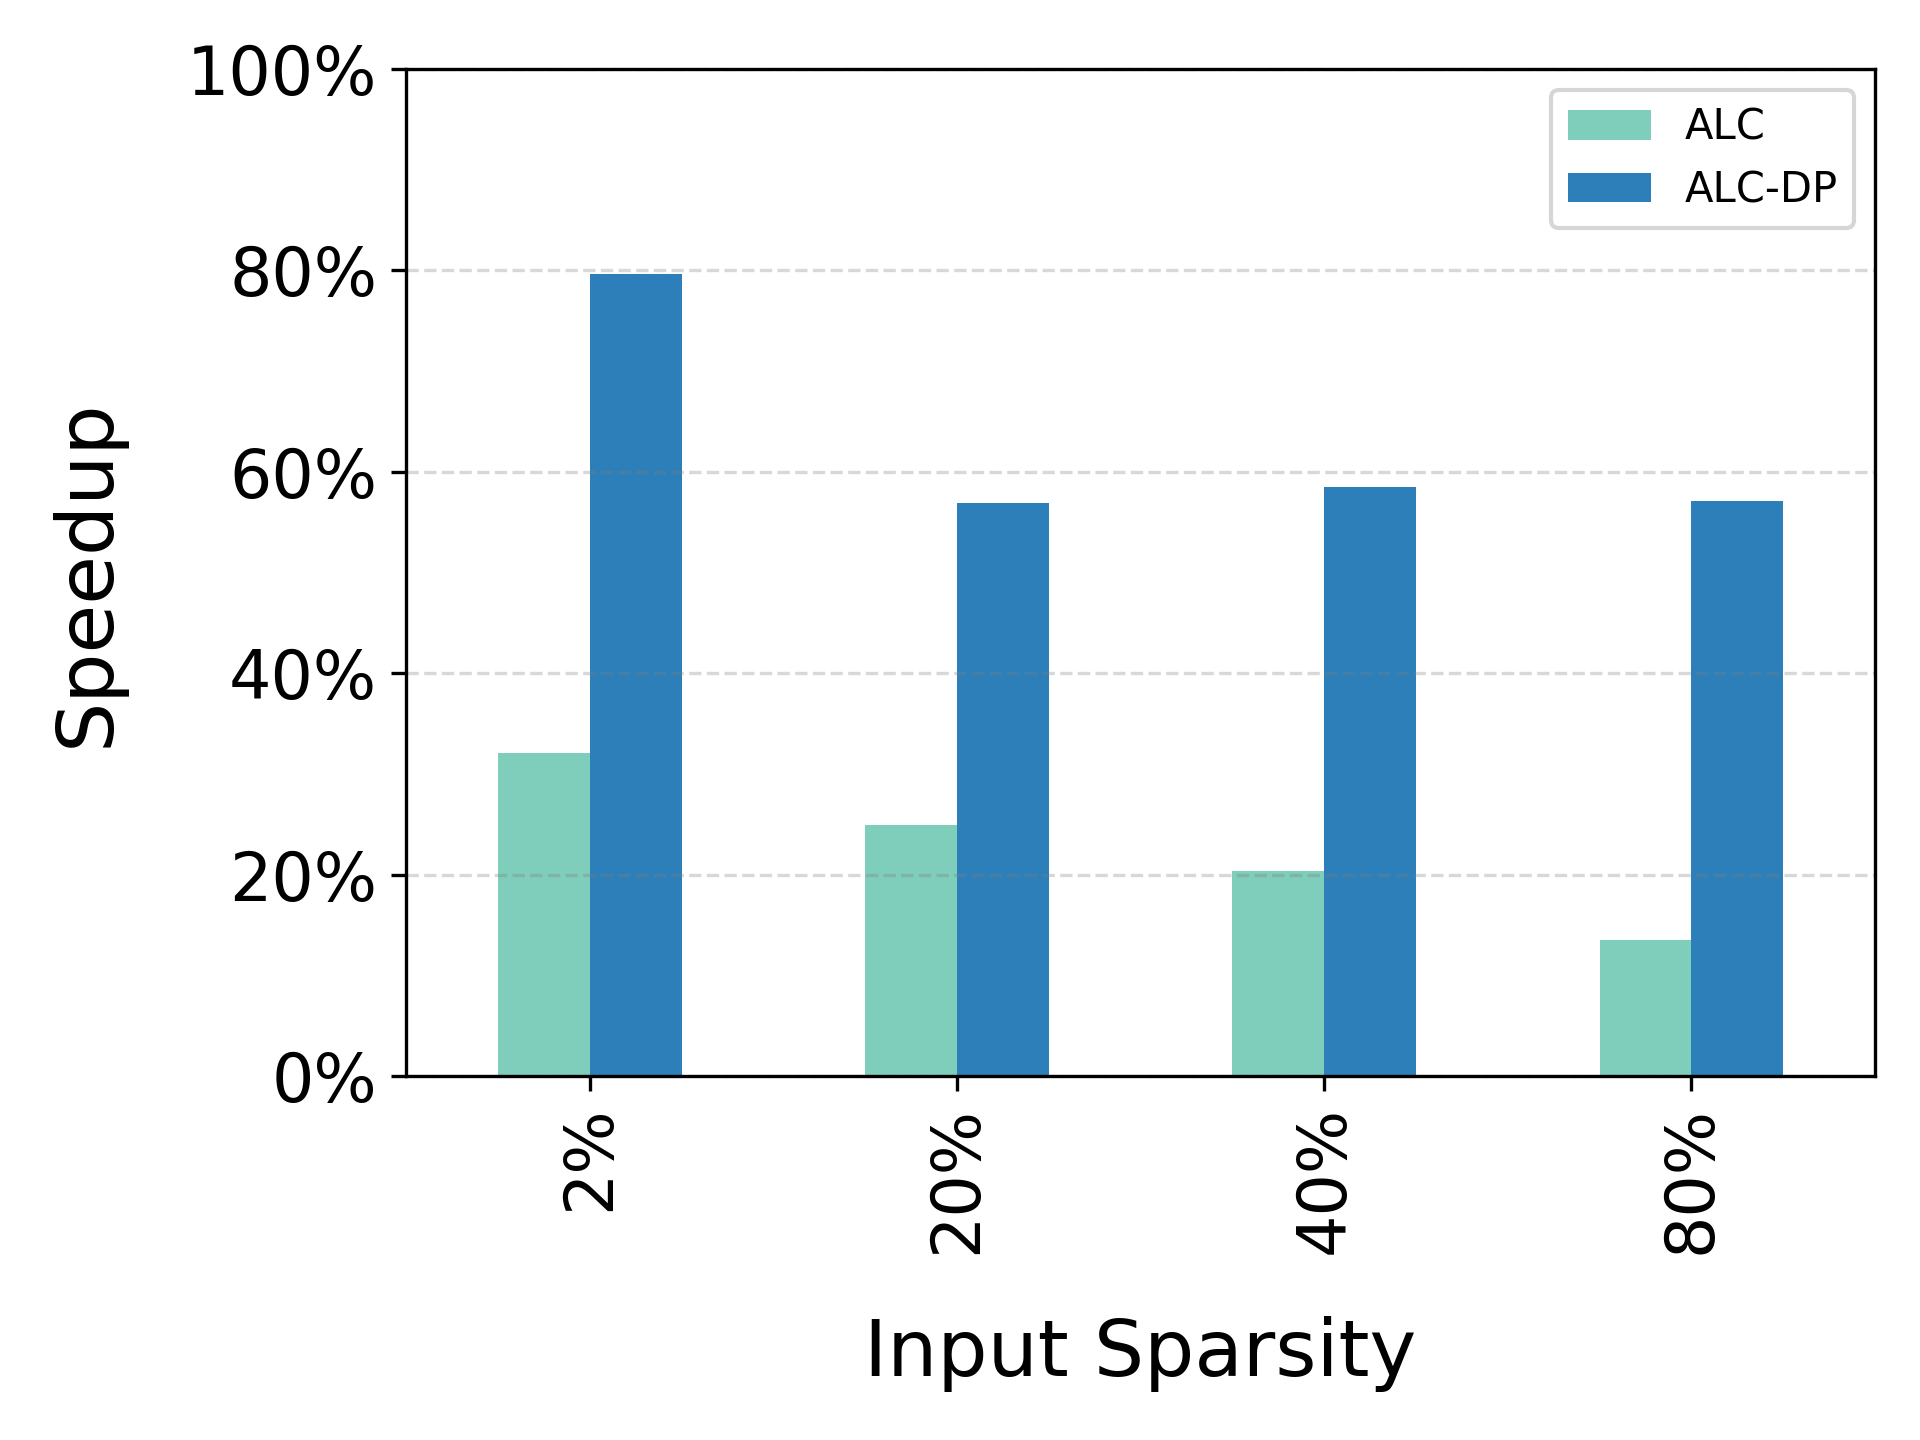
\includegraphics[width=\textwidth]{Figures/Evaluations/if_then_else_few_scatter_speedup.png}
    \caption{Speedup over \scalar (non-vectorized code).}
     \label{fig:if-then-else-few-scatter-speedup}
  \end{subfigure}%
  \begin{subfigure}{.499\textwidth}
        \centering
    \includegraphics[width=\textwidth]{Figures/Evaluations/if_then_else_few_scatter_speedup_over_ifConv.png}
    \caption{Speedup over If-Converted code}
    \label{fig:if-then-else-few-scatter-xppedup-over-ifConv}
  \end{subfigure}
  \begin{subfigure}{.499\textwidth}
    \centering
    \includegraphics[width=\textwidth]{Figures/Evaluations/if_then_else_few_scatter_instrcutions.png}
    \caption{Reduction in number of executed instructions (w.r.t \scalar).}
    \label{fig:if-then-else-few-scatter-inst}
  \end{subfigure}%
  \begin{subfigure}{.499\textwidth}
        \centering
    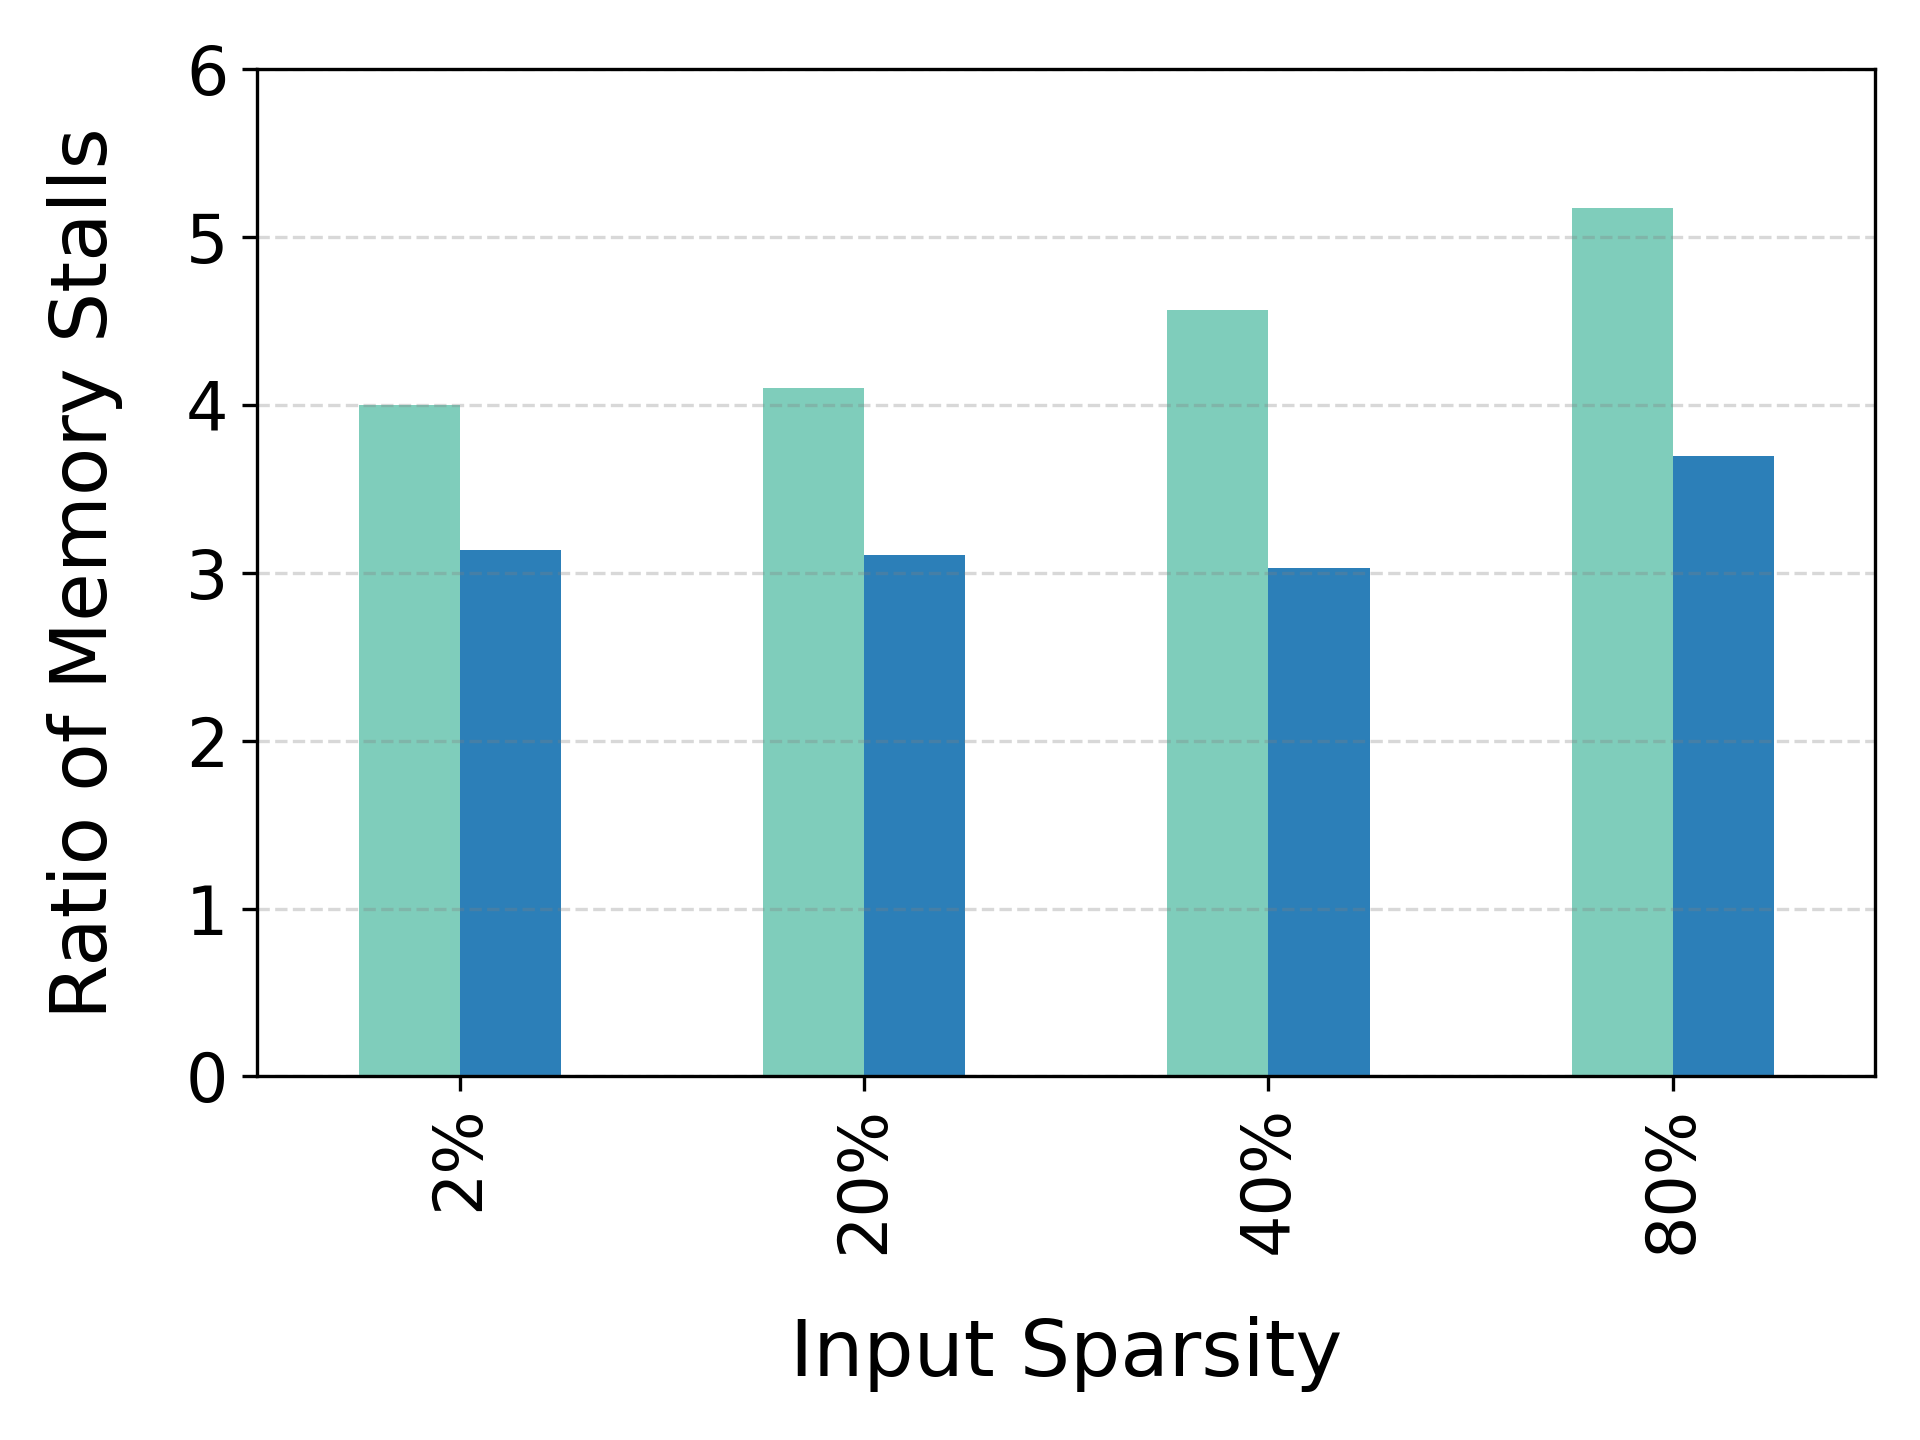
\includegraphics[width=\textwidth]{Figures/Evaluations/if_then_else_few_scatter_mem_stalls.png}
    \caption{Percentage of cycles stalled due to memory.}
    \label{fig:if-then-else-few-scatter-mem-stalls}
  \end{subfigure}
  
  \caption{Data Permutation Performance in the presence of Fewer Scatter Instructions}
  \label{fig:if-then-else-few-scatter}
\end{figure*}

\begin{figure*}[t]
  \begin{subfigure}{5cm}
    \centering
    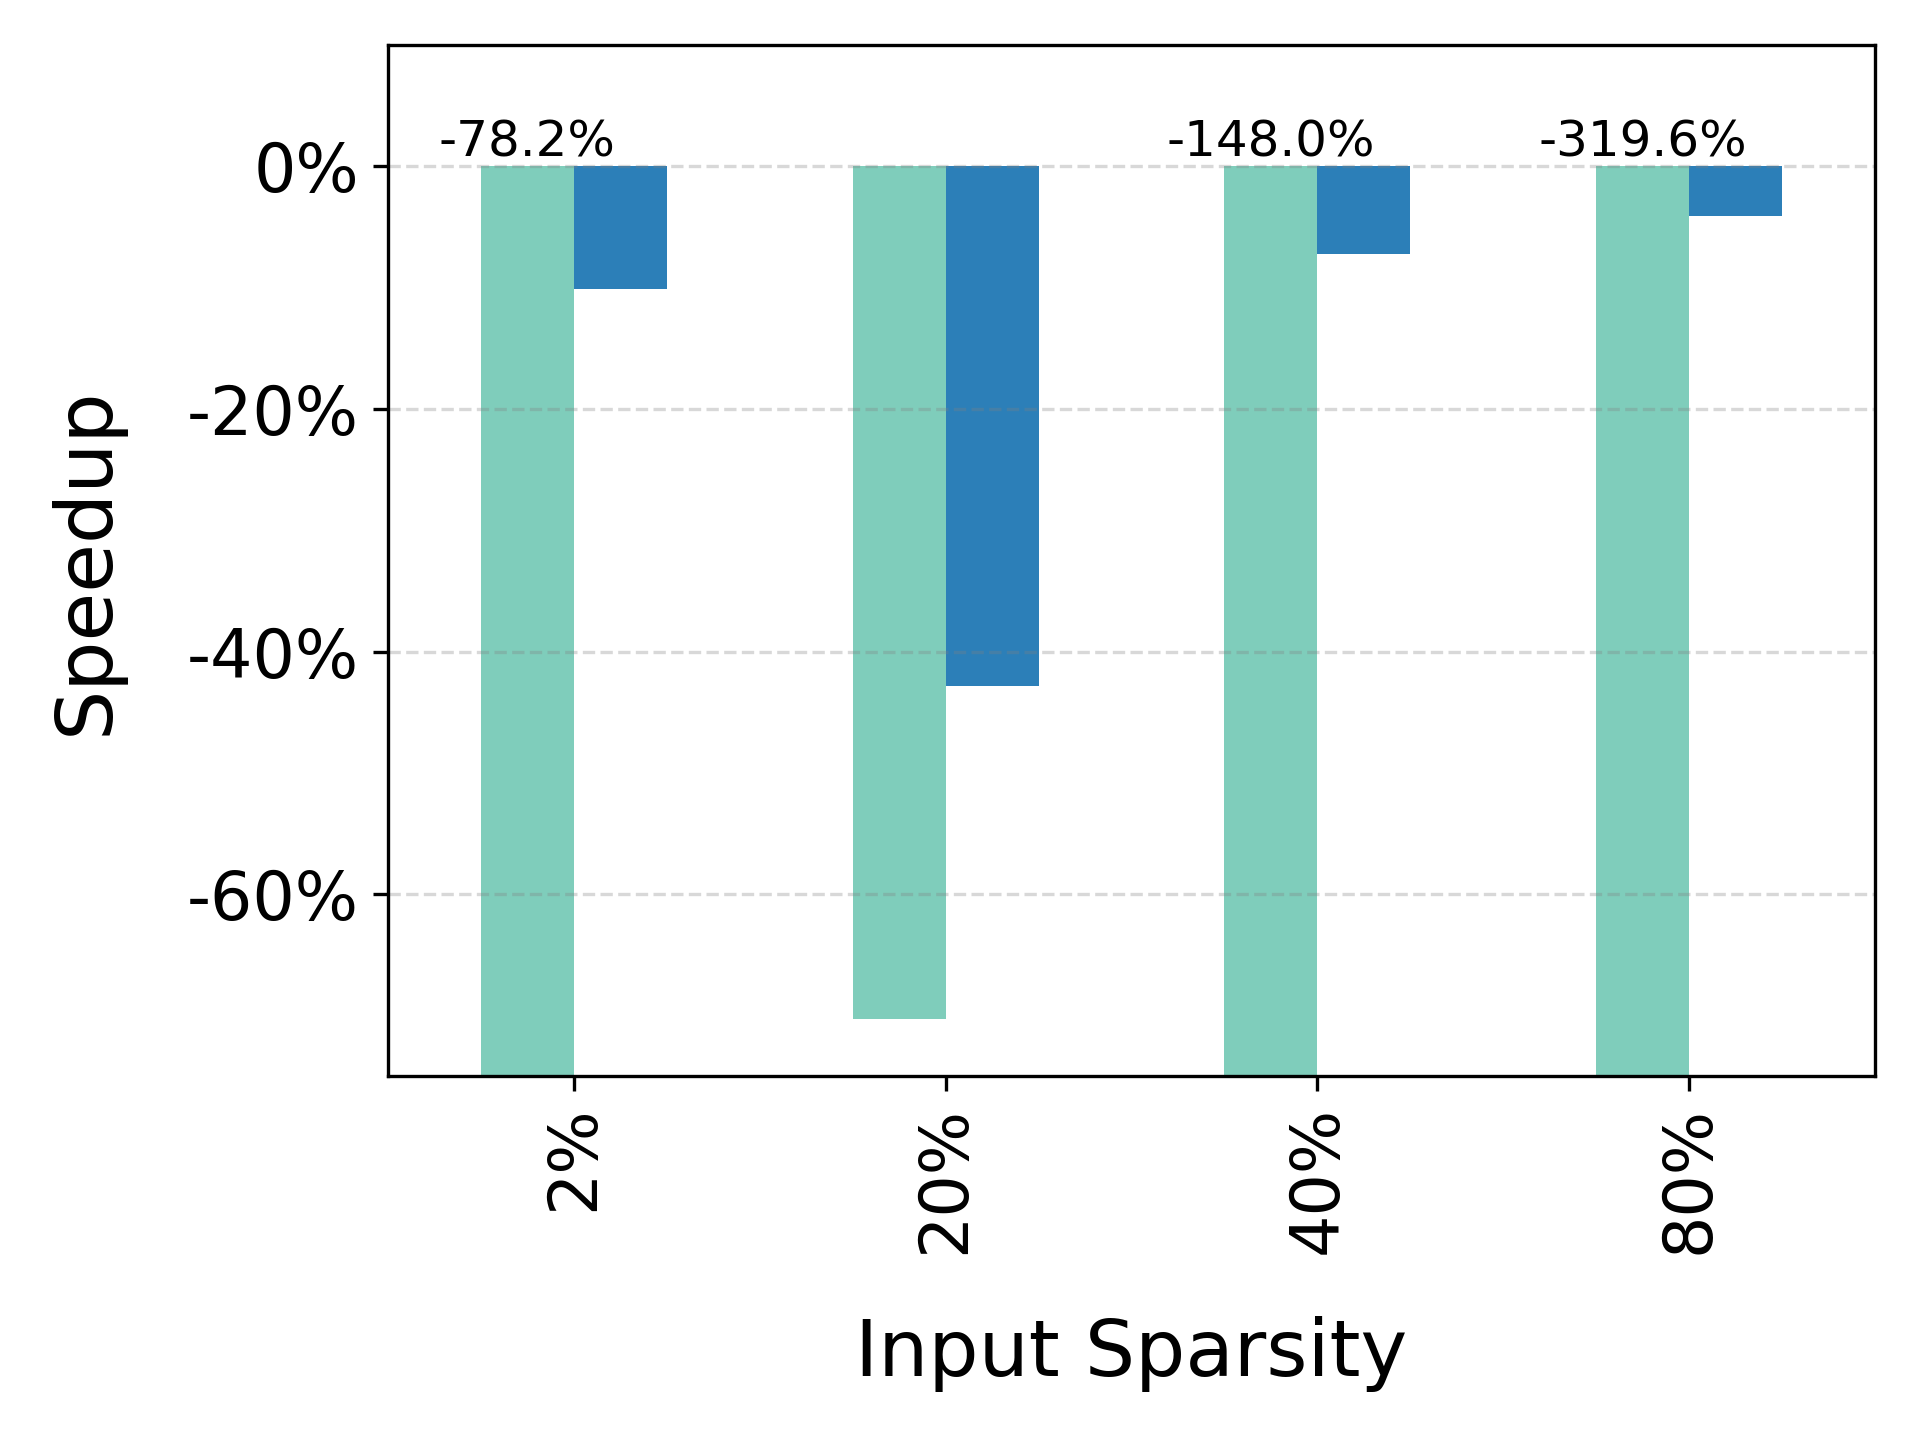
\includegraphics[width=\textwidth]{Figures/Evaluations/chart.png}
  \end{subfigure}
  \begin{subfigure}{.499\textwidth}
    \centering
    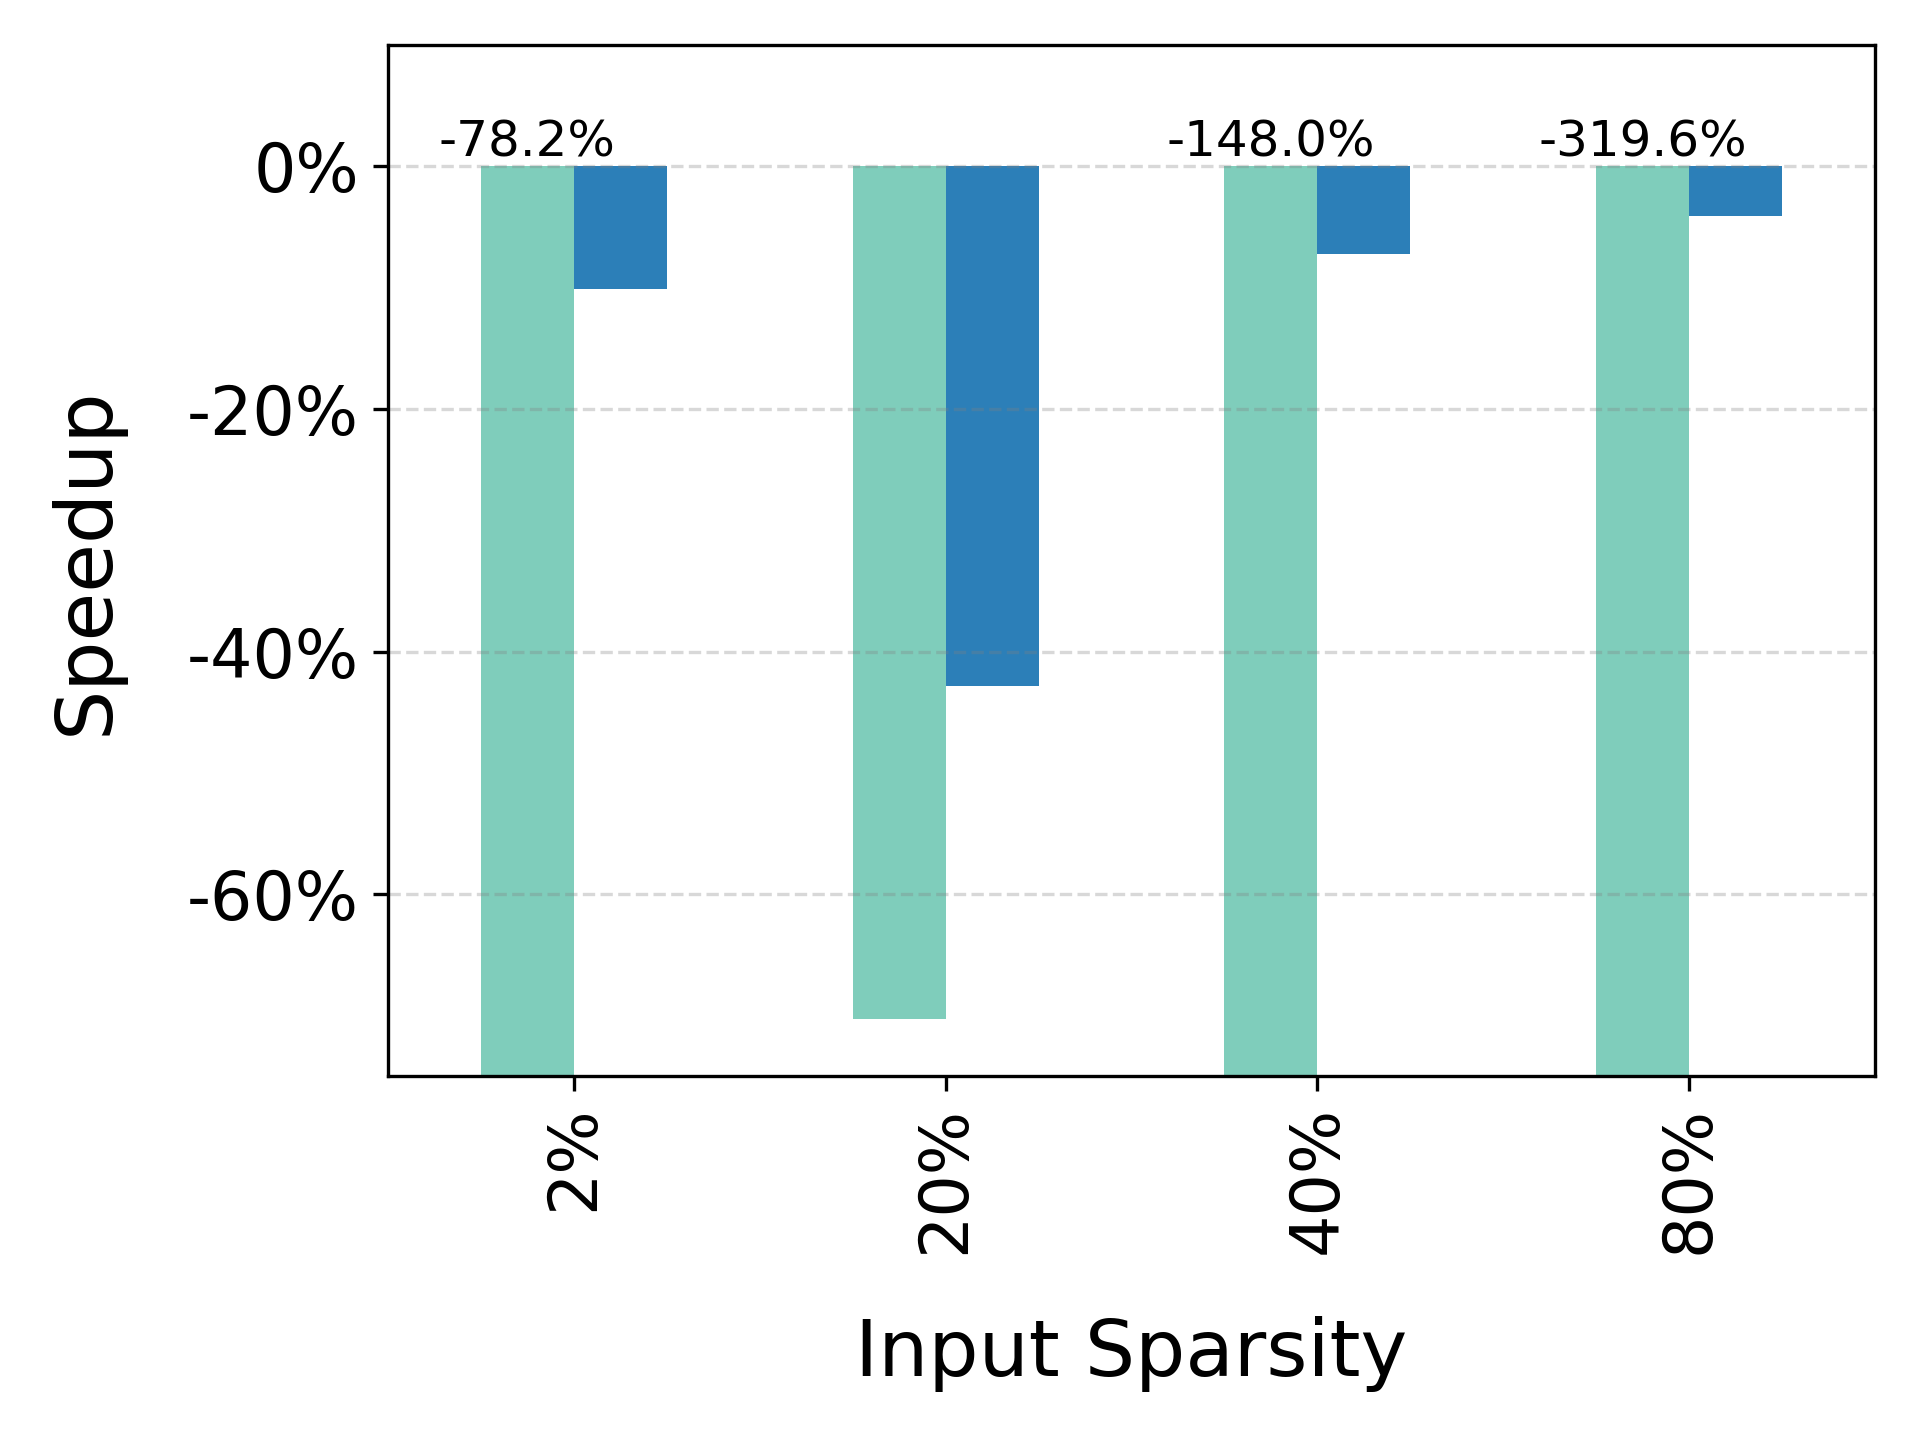
\includegraphics[width=\textwidth]{Figures/Evaluations/chart.png}
    \caption{Speedup over \scalar (non-vectorized code).}
     \label{fig:if-then-else-few-scatter-speedup}
  \end{subfigure}%
  \begin{subfigure}{.499\textwidth}
        \centering
    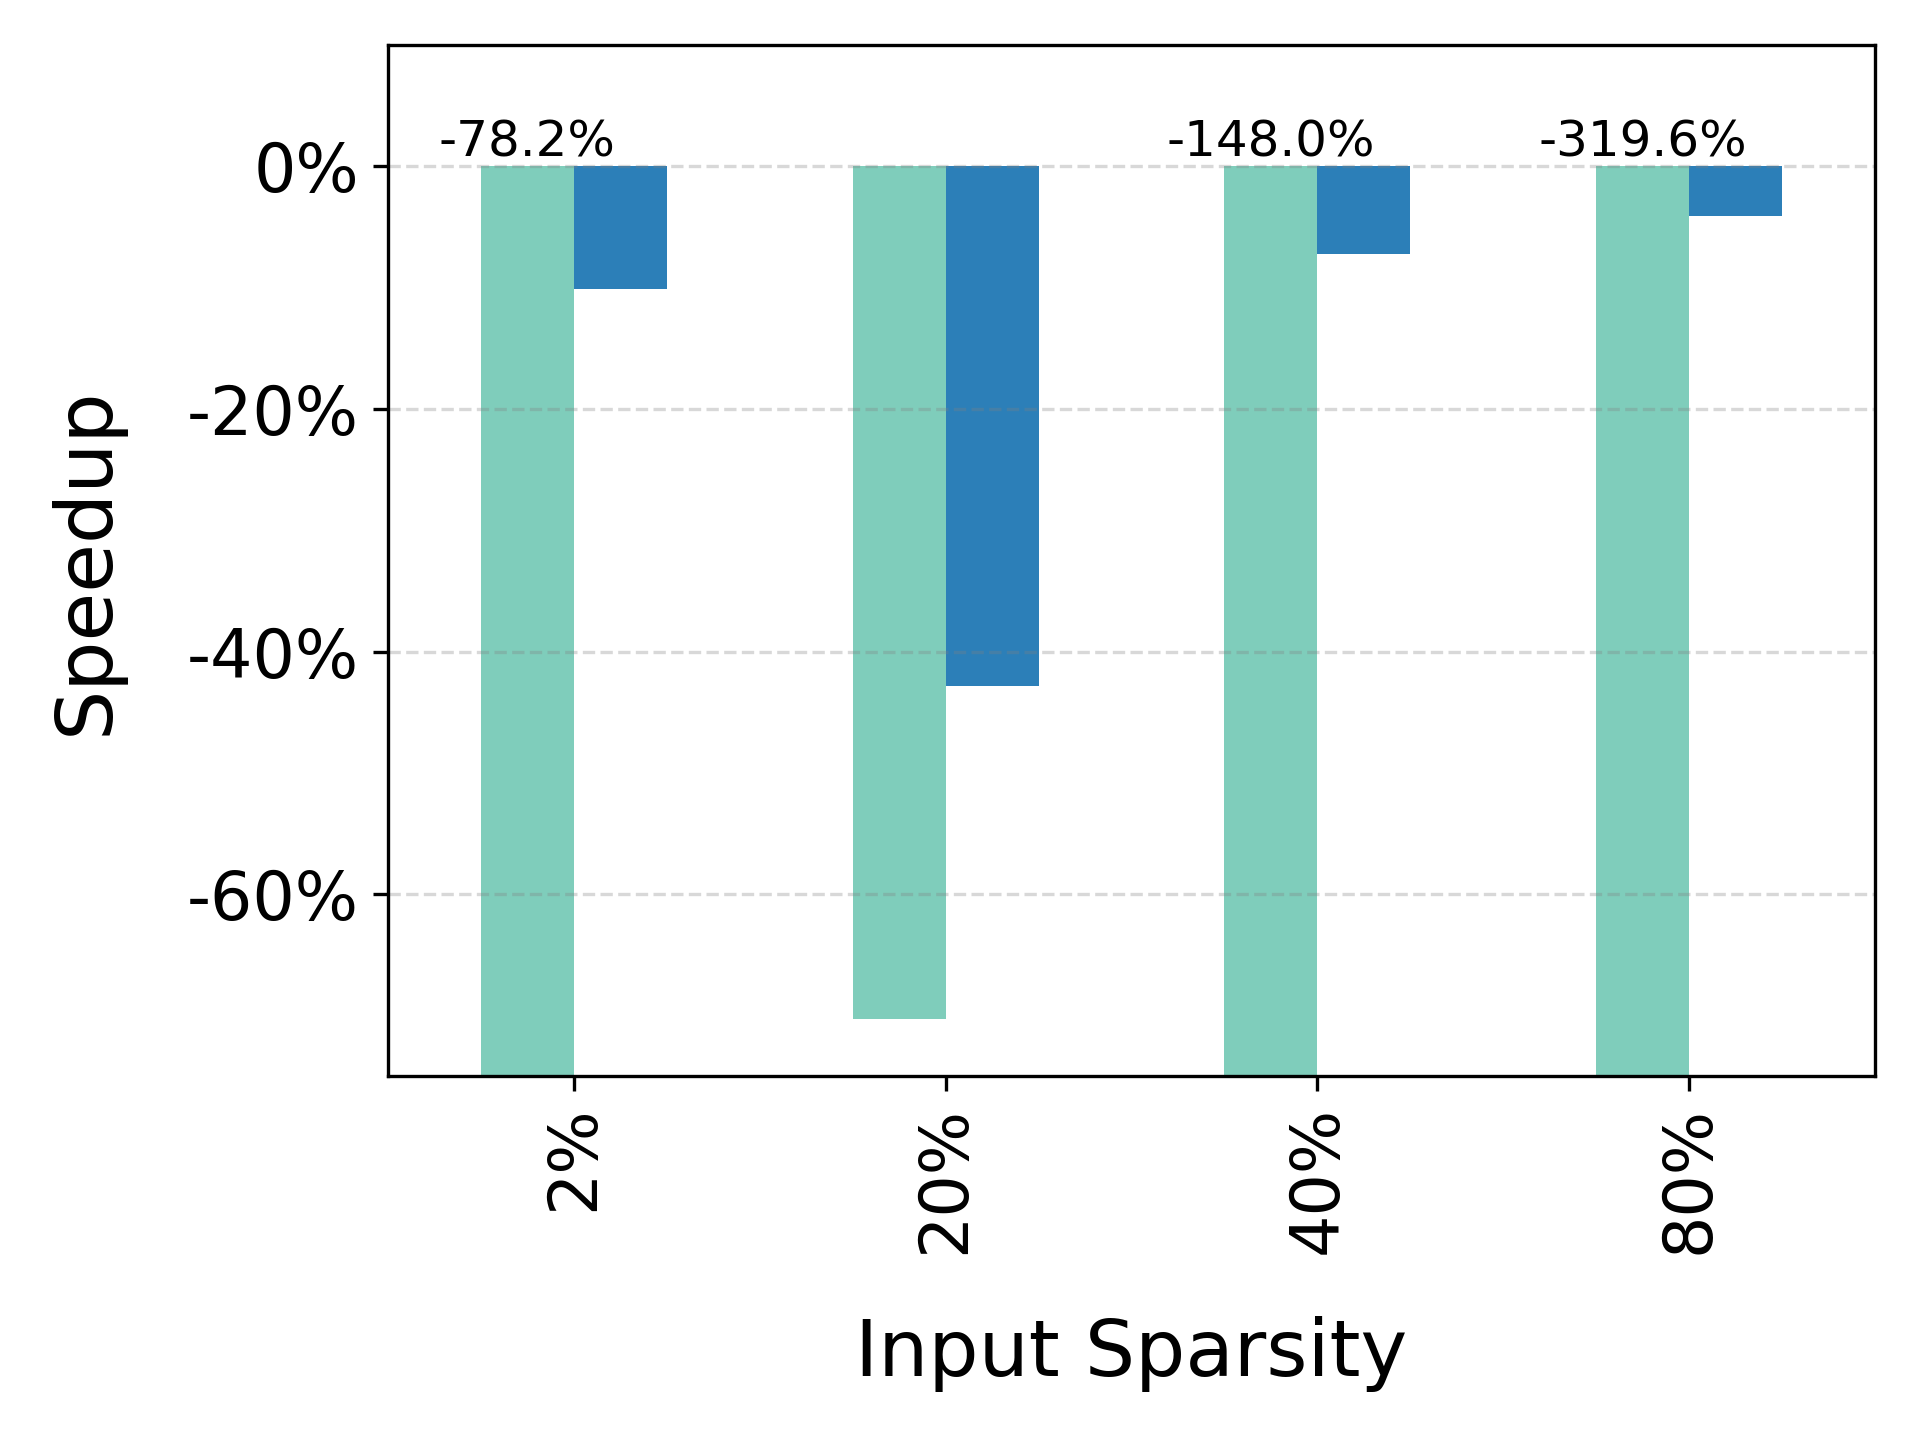
\includegraphics[width=\textwidth]{Figures/Evaluations/chart.png}
    \caption{Speedup over If-Converted code}
    \label{fig:if-then-else-few-scatter-xppedup-over-ifConv}
  \end{subfigure}
  \begin{subfigure}{.499\textwidth}
    \centering
    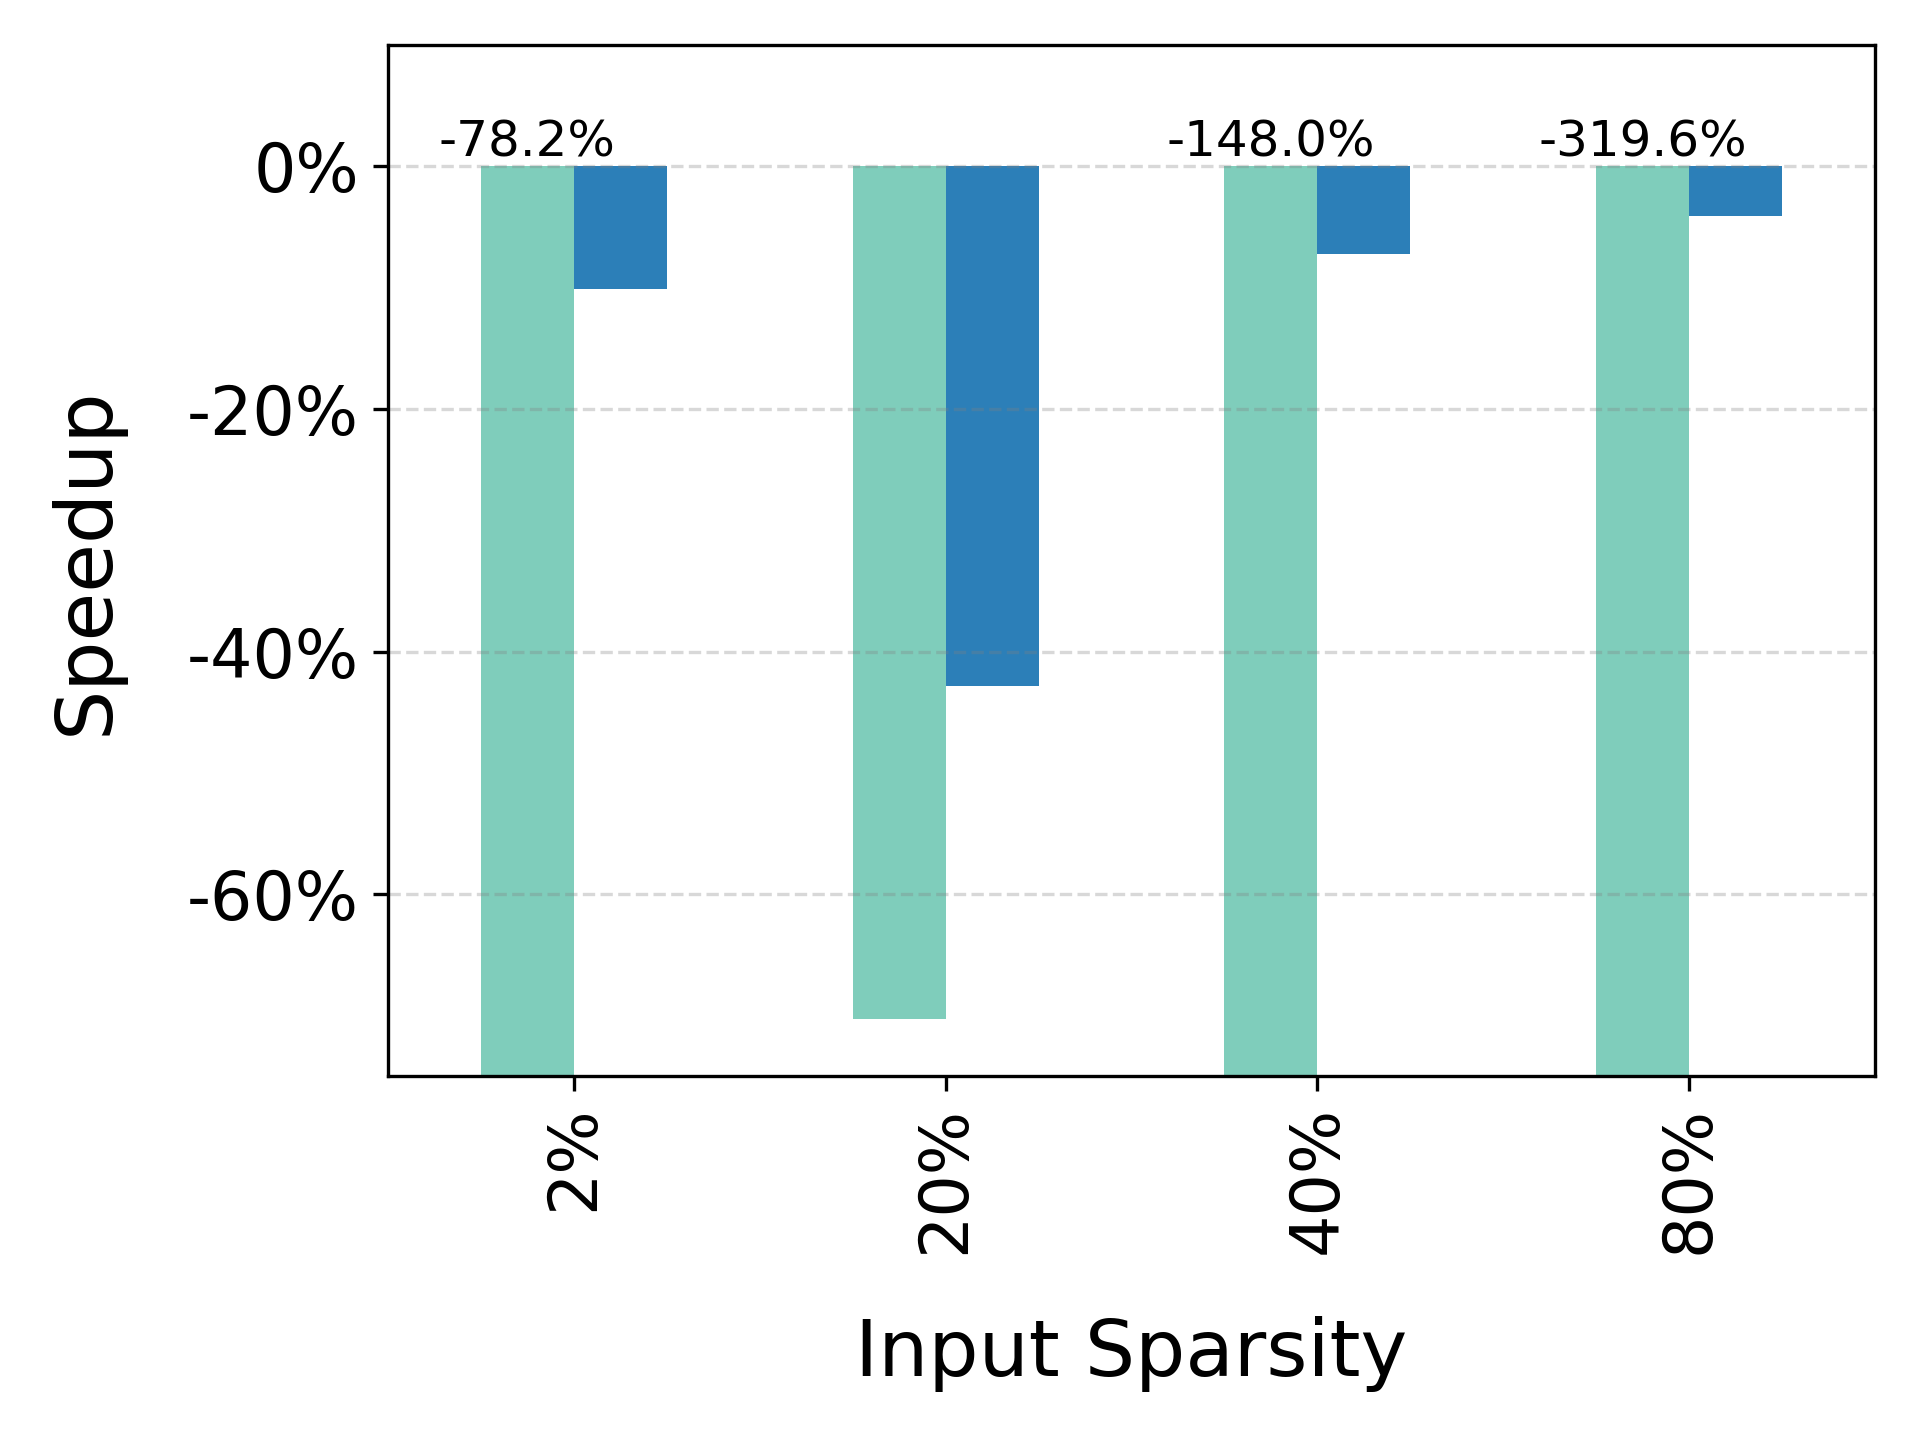
\includegraphics[width=\textwidth]{Figures/Evaluations/chart.png}
    \caption{Reduction in number of executed instructions (w.r.t \scalar).}
    \label{fig:if-then-else-few-scatter-inst}
  \end{subfigure}%
  
  \caption{Data Permutation Performance in the presence of Fewer Scatter Instructions}
  \label{fig:if-then-else-few-scatter}
\end{figure*}

% ######  ATTENTION #############
% The content above was left as a reference and is not going to be used for the paper.
% ######  ATTENTION #############
\fi